\documentclass[12pt, a4paper]{article}
\usepackage[a4paper, margin=1in]{geometry} %adjust margins
\usepackage{cite} %citation formatting
\usepackage{array}
\usepackage{graphicx}
\usepackage{longtable}
\usepackage{etoolbox}
\usepackage{subcaption}
\usepackage{float}
\usepackage{amsmath}
\usepackage{mathtools}
\usepackage[nottoc]{tocbibind}
\usepackage[intoc]{nomencl} %nomenclature in table of contents
% \usepackage{subfig} %for subfigures organized as grids

% \usepackage{subfig} 
\usepackage{multirow} %for having cell spanning multiple rows in tabular

\usepackage{pdfpages} %including front page

\usepackage{setspace} %1.5 spacing
\setstretch{1.5}

%for clickable table of contents
\usepackage{hyperref}
\hypersetup{
    colorlinks,
    citecolor=black,
    filecolor=black,
    linkcolor=black,
    urlcolor=black
}

%define command for symbol denoting "average of"
\newcommand*\mean[1]{\bar{#1}}

%paragraph spacing and indentation
\setlength{\parindent}{0em}
\setlength{\parskip}{1em}

%counter for numbering the rows of tables
\newcounter{rowcntr}[table]
\renewcommand{\therowcntr}{\thetable.\arabic{rowcntr}}
% A new columntype to apply automatic stepping
\newcolumntype{N}{>{\refstepcounter{rowcntr}\therowcntr}c}
% Reset the rowcntr counter at each new tabular
\AtBeginEnvironment{tabular}{\setcounter{rowcntr}{0}}

\makenomenclature

\begin{document}

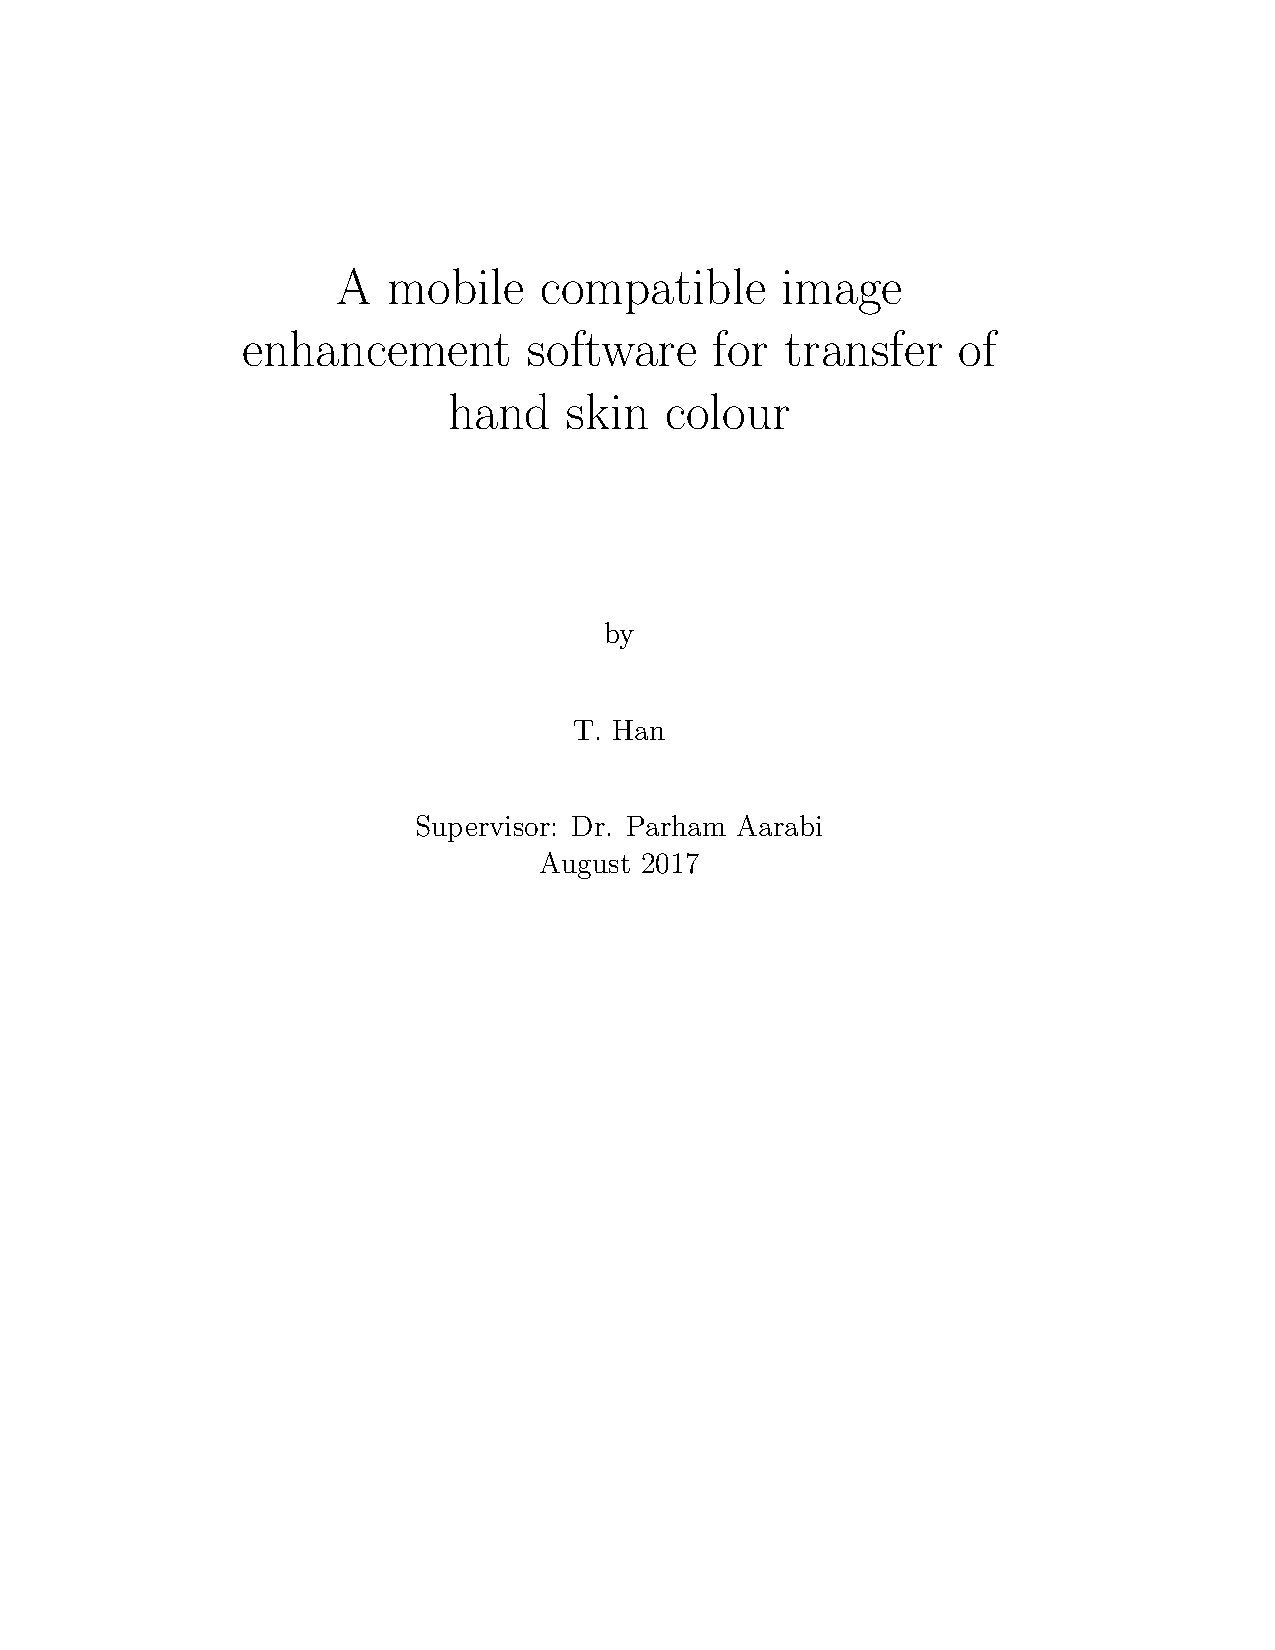
\includepdf{frontcover}

\renewcommand{\thepage}{\roman{page}}% Roman numerals for page counter
\setcounter{page}{1}

\section*{Abstract}
In the make up, beauty, and garment industries, there has been a growing trend to personalize images of models to take on the user's own bodily features in order to allow for users to better visualize products worn on themselves when making a purchasing decision. Specifically for this project, we have a nail polish virtual try-on mobile application that demonstrates nail polish colours on a video of a model hand of mid-toned skin colour, and our goal was to develop a software that would be able to tailor this video to each user by automatically adjusting the skin colour of the hand within each frame of the video to the user's skin colour. We developed an algorithm in C++ using OpenCV libraries and tested the effect on several hand images of various skin colours. We iterated through several different versions of the algorithm and determined that the best results are yielded by using an adjustment of the $rgb$ colours to match the average skin colour exactly to the target image, while proportionally fading off the adjustment based on distance to the average. Our results appear realistic on smaller skin colour changes but not on large skin colour changes. Future work would better address this and also test on a wider range of images and video frames, as well as optimize the algorithm for a mobile application.

\pagebreak

\section*{Acknowledgements}
Acknowledge persons and/or supporting agencies in a single-spaced paragraph in block form in centre of separate page.
\pagebreak

\tableofcontents
\pagebreak

\listoffigures
\listoftables
\pagebreak

\renewcommand{\nomname}{List of Symbols}
\printnomenclature
\pagebreak

\renewcommand{\thepage}{\arabic{page}}% Roman numerals for page counter
\setcounter{page}{1}

\section{Introduction}
%introduction
The modern shopping experience for cosmetics and garments increasingly takes place online and digitally. Since this means that the consumer or user often does not have direct, physical access to products for assessment before purchasing, many \textit{virtual try-on} applications have been developed to provide users with virtual experiences of 

digitally modify the images of models to take on the appearance of the user \cite{zhang_2017_try} \cite{shilkrot_2013_garment, li_2015_replace}.

% The physical differences between ourselves and a model means that we often cannot judge based on the appearance of a product worn by a model how that product will actually look on ourselves. Ideally, to help us, the users, make better informed purchasing decisions, the model demonstrating the product should be customized to each user. To achieve this, there are already many applications developed for virtually trying on products in the beauty, cosmetics and garment industries which digitally modify the images of models to take on the appearance of the user \cite{zhang_2017_try} \cite{shilkrot_2013_garment, li_2015_replace}.
%better describe "virtual try-on?"

Our project is concerned with improving a virtual try-on application that demonstrates different nail polish colours on a video of a generic model hand. We would like to edit this demo video so that the model appears to have the user's exact skin colour, to help the user better determine whether the nail polish colours look pleasant on the user's own hand. While it is possible to manually prepare a series of demo videos with models of a range skin colours, preparing even a single video for virtual try-on is an extremely time intensive task. Moreover, each person has a particular skin colour and it's preferable to be able to tailor the video exactly to the skin colour of the user while the user is using the app.

To address these challenges, we propose developing an algorithm to incorporate into the app that quickly and automatically performs the image editing task while the user is using the app. The user should be able to provide an image of their own hand as input, and the video of the model hand should be convincingly and accurately modified to having the skin colour of the provided user image. A wide range of user skin colours should be supported by a single model of mid-toned skin, and the process should be able to run quickly on a mobile device, such that the user notices no significant time lag to see the resulting video frames upon inputting their own skin colour.

Currently, we aren't aware of an existing algorithm that satisfies all our specific requirements. While there has been a large body of work done addressing transfer of colour between images in general \cite{reinhard_2001_transfer, pitie_2005_pdf, chen_2014_propagation, chang_2015_palette, zhang_2017_decomposition}, only a smaller set of work specifically addresses transfer of skin colour \cite{yin_2004_transfer, seo_2005_transfer, yang_2017_semantic}. All such studies address face skin colour rather than hand skin colour, which often means that more of the study is devoted to handling colour transfer of different, more complex aspects of the face \cite{yang_2017_semantic}. Skin colour transfer is also used as parts of other, more general imaging processing applications, but in those cases, since the skin colour transfer is often only a small part of the whole process, the algorithm used is often relatively simple and not heavily designed for achieving accuracy to the user skin colour \cite{shilkrot_2013_garment, li_2015_replace}. In the related field of skin colour enhancement applications, the methods used often are not meant to make large changes to the user skin colour \cite{aradhye_2009_enhancement, lee_2010_mobile}. Finally, algorithms developed by most of the prior studies do not appear to be meant for use with the limited resources on a mobile device. We discuss these previous studies of methods of skin colour transfer in detail in section \ref{sec:academic_work}.

% Our goal is to develop a mobile compatible recolouring algorithm that would satisfy our requirements. As sub-objectives, we would like to first develop an effective algorithm and then optimize the algorithm's running time. We will focus solely on achieving convincing colour transfer in the algorithm, and assume that the location of the skin in the images are already determined by an another process. 

% For developing and testing the algorithm, we will be using the OpenCV library in C++. OpenCV has a wide range of image processing tools and code in C++ should be easy to optimize and port to mobile platforms. We will develop the algorithm on a desktop computer, to allow for faster and easier testing, before we port the code to mobile. Our approach will be to test different algorithms on variety of hand images, starting with a naive approach and developing improved versions of the algorithm based on the results after each each iteration.

\subsection{The goals, constraints and requirements for an effective skin colour transfer algorithm}
Our project is intended to manipulate image frames in a video of a model hand demonstrating nail polish product so that the model hand takes on the user's skin colour. The images we must process will mostly consist of the back of a single hand shown prominently in the image. We expect image sizes the algorithm should be able to handle to be at least 800 by 800 pixels in size. We show an example of the desired output of our algorithm in Table \ref{tab:our_demo}.

\begin{table}[H]
	\centering
	\caption{Example of our desired output given a source (the model) and a target image (from the user) \label{tab:our_demo}}	
\begin{tabular}{|c|c|c|}
	\hline
	Source & Target & Output \\ 
	\hline
	  \begin{minipage}{.29\textwidth}
	    \includegraphics[width=\textwidth,height=\textheight,keepaspectratio]{../inputs/hand_brown.jpg}
	  \end{minipage} & 
	  \begin{minipage}{.29\textwidth}
	    \includegraphics[width=\textwidth,height=\textheight,keepaspectratio]{../inputs/hand_light.jpg}
	  \end{minipage} & 
	  \begin{minipage}{.29\textwidth}
	    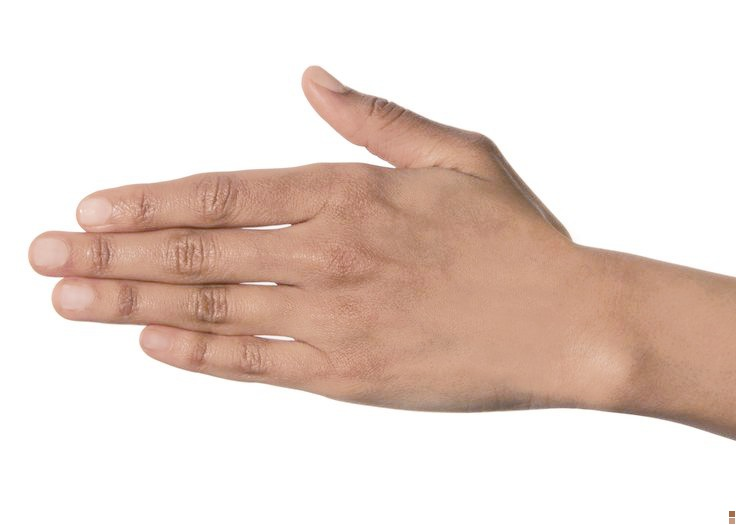
\includegraphics[width=\textwidth,height=\textheight,keepaspectratio]{../rc_test/outputs/20170524_prop_corr_1p1_ave_100/hand_brown_to_hand_light.jpg}
	  \end{minipage} \\
	\hline
 \end{tabular}
 \end{table}

To narrow the scope of our project, we will not include skin detection as part of this project and assume that our algorithm is already given a mask of the skin areas of all the images. We will focus solely on the transfer of the hand skin colour. 

Based on our goals and the nature of our project, we list below several constraints and design paradigms against which we will evaluate our algorithm:

\textbf{Compatible with mobile device:} Our algorithm is ultimately intended to support an application on a mobile device, so we must ensure that our code is portable to mobile devices and that the algorithm we develop can operate quickly with the limited resources of a mobile device so that the user will be able to see near-instant results.

\textbf{Fully automatic:} Since the goal of our project is for a commercial user to be able to change the model to his or her own skin colour, our algorithm cannot rely on any user input to perform the image editing and should able to accept only an image containing the user's own hand as the target image to transfer the colour of the model hand to.

\textbf{Realistic skin colour transfer:}
Since the goal of our project is to perform skin colour transfer for model images that are meant to demonstrate cosmetic products to users, and the results are meant to invoke for the user the impression that the user's own hand is wearing the product, our final images must look as realistic as possible to avoid a displeasing, uncanny valley effect. Furthermore, the images we process will be large and feature the skin on the back of a hand very prominently, so we can expect that unrealistic flaws in our result will be very noticeable the user.

\textbf{Accurate skin colour transfer:} 
Since the entire goal of nail polish try-on application is to demonstrate to the user how a particular shade of nail polish will appear on his or her own hand, we must ensure that the results of the algorithm, more than looking pleasing to the user, actually matches the skin colour sample provided by the user exactly.

\textbf{Wide range of colour transfer:} Since the goal of the project is to reduce the number of nail polish try-on videos of different skin colours needed and since users may have a wide range of skin colour and should all be supported, our algorithm needs to be able to transfer the skin colour of a mid-toned hand to as wide a range of skin colour as possible.
\pagebreak

\section{Background and Literature Review}
%literature review
\section{Related prior work}

Relevant prior work fall into four rough categories. There is a large body of work on the subject of general automatic colour transfer and colour grading by example, transfering the ``style" or specific colours in an example image to another image. There have been several prior attempts at transfering specifically images wherein skin colour is prominent, and these we will discuss in detail. There are also several examples of practical application of skin transfer algorithms, where different application demonstrate practical uses of usually relatively simple skin transfer algorithm that is part of a larger project; we will discuss several of these projects. Finally, there is the field of skintone enhancement software, where algorithms are usually intended to adjust the user skin colour towards a more pleasing tone and not to a specific target colour. We include the latter because unlike the other categories of prior work there are several studies of adjusting skintone on a mobile device, which is part of the requirements for this project.

\section{Colour transfer by example image for general images}
Colour transfer refers to modifying the colours of an image to give it the desired appearance and style demonstrated by an example image, which we will refer to as the target image. Figure \ref{fig:color_transfer} illustrates an example of this effect.

There have been a wide range of work done in this area beginning with the seminal work of Reinhard et al. in 2001 \cite{reinhard_2001_transfer}. 

While these techniques are interesting possibilities to try when transfering human skin colour, because the these prior studies are all concerned with different problems that can arise with general images but not specifically for human skin colour, studies that specifically relate to human skin colour demonstrate that the general colour transfer techniques can be improved upon.

\section{Transfer of human skin colour}
Several studies have been done specifically on the transfer of human skin colour.

Seo et al. \cite{seo_2005_transfer} has a purpose closest to the purpose of this project, to transfer human skin colours. The authors show results that improve in realistic appearance compared to the Reinhard's algorithm.

%models the skin as ellipsoid distribution around vector, with another vector for specular reflection
%algorithm used - RGB space transform, division into bins and moving standard dev and mean while leaving details intact
%Results don't show range but we can possibly replicate and check?

It is not clear how fast the algorithm can run particularly on a mobile device, nor the range of colours that the algorithm can transform a single skin colour, and it is in these areas that our project will attempt to improve upon.

Yang et al. Performed the most recent study 


%explain theoretical concepts in context of thesis work; be clear and concise
%summarize relevant research to give understanding of current field
%analyze research in field to give deeper understanding of research question 
%indicate a path going forward



%photoshop
\subsection{Changing and matching skin colour in Photoshop}

Skin colour correction is a frequent problem encountered in photo retouching and there are a wide range of online video tutorials available documenting the methods artists use to manually adjust human skin tone in individual images using Adobe Photoshop, a widely used commercial image manipulation software. The purposes of these videos include giving the subject of an image the appearance of a tan, matching the skin tone of the subject to a desired skin tone on another individual, or matching the skin tone of a subject's face to the rest of the subject's body, which is often a slightly different colour \cite{photoshop:tan, photoshop:match_other, photoshop:match_body}. Bearing in mind that techniques described by such tutorials expect artistic input from a human editor to acheive the results and are therefore not entirely aligned with the purposes of this project, it is useful to study these methods because the results achieved are usually extremely realistic and aesthetically pleasing and should be a standard that the algorithm developed in this project strives towards. We therefore surveyed a number of these videos and summarize below the techniques of some of the most relevant videos.

\subsubsection*{Summary of Photoshop techniques}

Shaver demonstrated how to change a person's skin colour from dark to light \cite{photoshop:obama}, which is an impressively wide range to change. Shaver used levels and curves, which are tools that manipulate the $rgb$ colour histogram of the image, to increase brightness to an extent, then performed further brightening by using a grey scale conversion to brighten the skin area of a black and white image and then using the luminosity blend mode to place the colour back into the image. We show the results acheived in Table \ref{tab:obama_demo}.

\begin{longtable}{|c|c|}
    \caption{Screen captures from Photoshop tutorial for changing skin colour from dark to light. \label{tab:obama_demo}}\\
    \hline
    Original & Result \\
    \hline
  \begin{minipage}{.29\textwidth}
    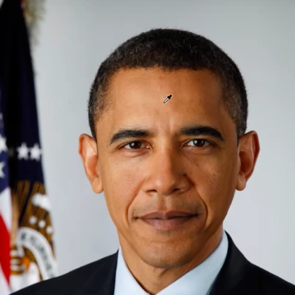
\includegraphics[width=\textwidth,height=\textheight,keepaspectratio]{images/obama_orig}
  \end{minipage} & 
  \begin{minipage}{.29\textwidth}
    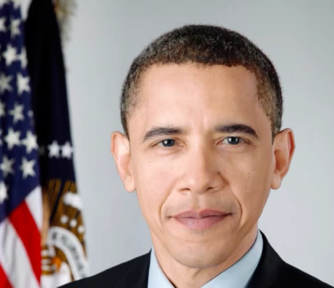
\includegraphics[width=\textwidth,height=\textheight,keepaspectratio]{images/obama_res}
  \end{minipage} \\
    \hline
\end{longtable}

Phlearn demonstrated an effect in the reverse direction by demonstrating a technique for giving the model the image appearance of a dark tan \cite{photoshop:tan}. The highlights and shadows of the image are adjusted separately by using the ``blend if" function of Photoshop, which blends in an effect only if the original pixel is above a certain threshold of brightness.

Phlearn also demonstrated a method for matching the skin colour of body and face in an image where the two appear mismatched \cite{photoshop:match_body}. The author sampled a range of colours from the body and adjusted the face with the levels tool for each colour channel. We show the results acheived in Table \ref{tab:match_body_demo}.

\begin{longtable}{|c|c|c|}
    \caption{Screen captures from Photoshop tutorial for matching the skintones of face and body. \label{tab:match_body_demo}}\\
    \hline
    Original & Target & Result \\
    \hline
  \begin{minipage}{.29\textwidth}
    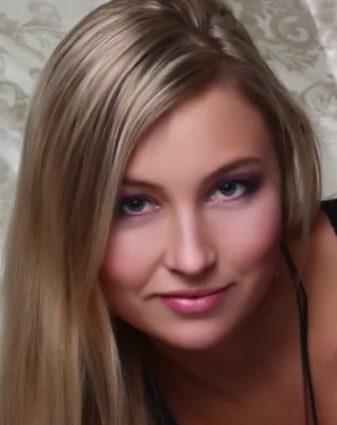
\includegraphics[width=\textwidth,height=\textheight,keepaspectratio]{images/match_body_orig}
  \end{minipage} & 
  \begin{minipage}{.29\textwidth}
    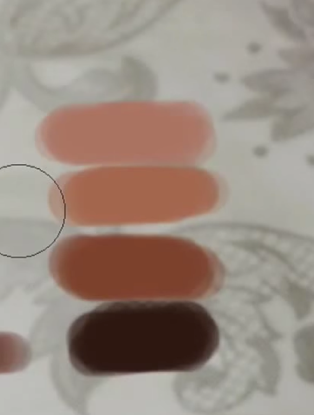
\includegraphics[width=\textwidth,height=\textheight,keepaspectratio]{images/match_body_targ}
  \end{minipage} & 
  \begin{minipage}{.29\textwidth}
    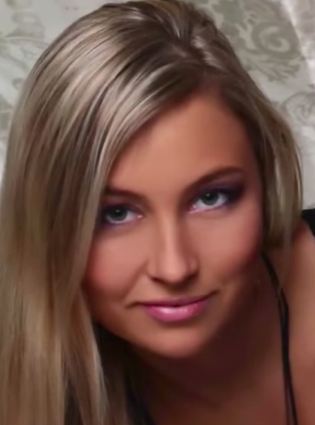
\includegraphics[width=\textwidth,height=\textheight,keepaspectratio]{images/match_body_res}
  \end{minipage} \\
    \hline
\end{longtable}

PiXimperfect demonstrated a method for matching skin colour in one portrait to another \cite{photoshop:match_other}. PiXimperfect first calculates the two average colours of the faces and uses the Photoshop curves tool to match the average colours of the original image to the target image. There must then be further adjustments by eye to change colour, brightness and contrast. Examples of the results from PiXimperfect is show in Table \ref{tab:match_other_demo}

\begin{longtable}{|N||c|c|c|}
    \caption{Screen captures from Photoshop tutorial for matching the skintones of portraits of different people. \label{tab:match_other_demo}}\\
    \hline
    \multicolumn{1}{|c||}{No.} & Original & Target & Result \\
    \hline  \label{row:photoshop_match_other_1} &
  \begin{minipage}{.29\textwidth}
    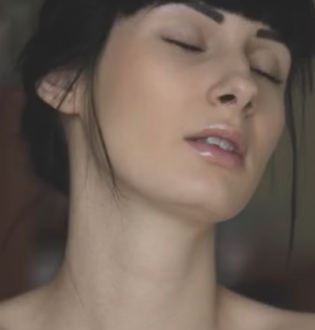
\includegraphics[width=\textwidth,height=\textheight,keepaspectratio]{images/match_other_1_orig}
  \end{minipage} & 
  \begin{minipage}{.29\textwidth}
    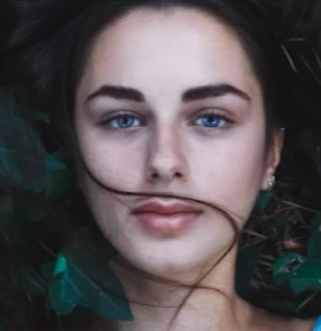
\includegraphics[width=\textwidth,height=\textheight,keepaspectratio]{images/match_other_1_targ}
  \end{minipage} & 
  \begin{minipage}{.29\textwidth}
    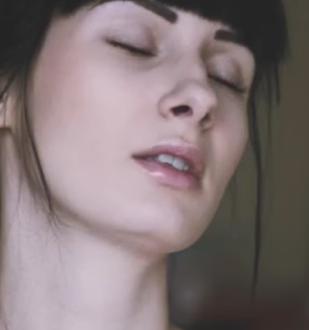
\includegraphics[width=\textwidth,height=\textheight,keepaspectratio]{images/match_other_1_res}
  \end{minipage} \\
    \hline  \label{row:photoshop_match_other_2} &
  \begin{minipage}{.29\textwidth}
    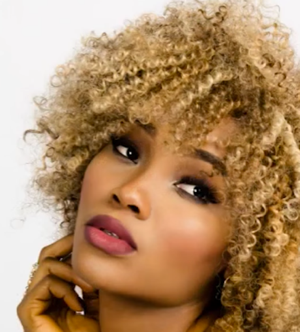
\includegraphics[width=\textwidth,height=\textheight,keepaspectratio]{images/match_other_2_orig}
  \end{minipage} & 
  \begin{minipage}{.29\textwidth}
    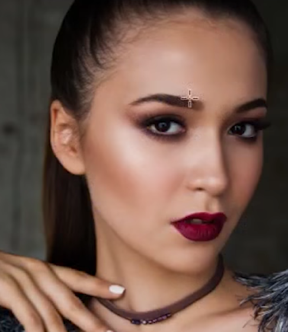
\includegraphics[width=\textwidth,height=\textheight,keepaspectratio]{images/match_other_2_targ}
  \end{minipage} & 
  \begin{minipage}{.29\textwidth}
    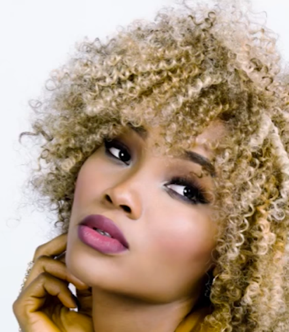
\includegraphics[width=\textwidth,height=\textheight,keepaspectratio]{images/match_other_2_res}
  \end{minipage} \\
    \hline
\end{longtable}

In summary, for most of the techniques surveyed, levels and curves are frequently used for small brightness adjustments \cite{photoshop:obama, photoshop:match_body, photoshop:match_other}, and often to reduce the vividness of the colour adjustments the saturation must be slightly decreased \cite{photoshop:obama, photoshop:match_body}. After all other effects are applied, the opacity of the overall effect is often reduced from 100\% for a more natural appearance \cite{photoshop:obama, photoshop:match_body}.

\subsubsection*{Limitations of Photoshop techniques}
Unlike the purpose of our project, the Photoshop techniques surveyed are not meant for automation. Instead, they are meant to be tailored to each specific image that a human is adjusting, and there are many junctures where the specific numerical amount of an adjustment often have to be judged by eye. While Photoshop has a method for automating processes using actions, the processes are meant for increasing ease of use by artists who can make additional adjustments and are familiar with the tool, rather than for use in commercial applications where the process is entirely automated \cite{photoshop:actions}.

Another limitation is that Photoshop operates at a higher level of abstraction than image processing software making use of libraries such as OpenCV. Image processing code has much more control over processes that can be applied to images, and the regions on the image that processes are applied to. 

Finally, some Photoshop effects may be proprietary and are of course limited to the platforms that Photoshop supports, while a program developed with a platform such as OpenCV can be made open source and adapted to uses on a variety of different platforms.

\pagebreak

\section{Hand Recolouration Algorithms}
%methods 
To accomplish the objective of recolouring the skin tone of a hand to a target colour, we wrote algorithms in C++ in Eclipse on OS X using OpenCV libraries. Eclipse is used to compile each iteration of the algorithm into a debug-mode executable program named Recolor. For ease of testing, as the algorithm is modified, we add more functionality to the Recolor program and retain the ability to use previous versions of the algorithm. We use a custom Python script to run new versions of Recolor from the terminal to test it. All of the relevant code and its versions are hosted on a git repository at github.com/tiantianhan/recolor

Recolor takes as input a hand image, a mask instructing it where to find the average skin colour of the hand, and a desired target skin colour. (Other flags and inputs are also used for testing purposes, see the Github repository readme file for a full description of the usage.) Recolor then outputs the processed image where the skin tone is adjusted to the target colour.

We iterated from simple to more complex algorithms, at each step testing the algorithm and evaluating the results. We tested progressive iterations on a set of hand images with varying skin tones. The images are are shown in Figure \ref{img:input_hands_1}.

%all images that are not test results will be copied to the images folder

\begin{figure}[H]
    \centering
    \begin{subfigure}[b]{0.20\textwidth}
        \includegraphics[width=\textwidth]{images/hand_dark}
        \caption{}\label{img:input_hands_1_dark}
    \end{subfigure}
    ~
    \begin{subfigure}[b]{0.20\textwidth}
        \includegraphics[width=\textwidth]{images/hand_brown}
        \caption{}\label{img:input_hands_1_brown}
    \end{subfigure}
    ~
    \begin{subfigure}[b]{0.20\textwidth}
        \includegraphics[width=\textwidth]{images/hand_light}
        \caption{}\label{img:input_hands_1_light}
    \end{subfigure}
    ~
    \begin{subfigure}[b]{0.20\textwidth}
        \includegraphics[width=\textwidth]{images/hand_pale}
        \caption{}\label{img:input_hands_1_pale}
    \end{subfigure}
    \caption{Different hand images used for testing}\label{img:input_hands_1}
\end{figure}

 For each test, we called the Recolor program to transform the image of one hand to have the skin tone of the hand in another image, then visually compared the processed image to the image of the target hand. We performed the process on all possible combinations of our test images, paying particular attention to the extreme cases, such as transforming from Figure \ref{img:input_hands_1_dark} to Figure \ref{img:input_hands_1_pale} and vice versa, as well as cases that start with a hand with mid-tone skin such as in Figure \ref{img:input_hands_1_brown} (as this is the most likely use case for applications that change the image of a model's hand to match a range of skin tones). We evaluated the resulting images subjectively, based on whether the processed hand looks believably like a hand naturally of that skin tone, and noted any flaws that we then attempted to correct with the next iteration of the algorithm.

In the following subsections we summarize the results of each algorithm and our evaluation of the results.

\subsection{Simple brightness addition / subtraction}
%boost algo
\subsubsection*{Algorithm}
To begin, we performed a simple addition of a value to each of the $RGB$ channels of the hand, such that the average colour of the hand in the processed image is equal to the average colour of the hand in the target image.

% \begin{equation} \label{eq:boost_algo}
% r' = r + \delta_r
% \end{equation}

% Where 

% \begin{equation*}
% \delta_r = \mean{r_t} - \mean{r}
% \end{equation*}

\begin{algorithm}[H]
\caption{Simple addition to $RGB$ channel.}
\label{eq:boost_algo}
\begin{algorithmic}
\State $T$ is the set of pixels in the target image, and $U
\State $\mean{C_T} \gets \Call{Mean}{\vect{C_T}(U)}$
\State $\mean{C_S} \gets \Call{Mean}{\vect{C_S}(V)}$
\For{each pixel $i$}
\State $\vect{C_O}(i) = \vect{C_S}(i) + (\mean{C_{T,U}} - \mean{C_{S,V}})$
\EndFor
\end{algorithmic}
\end{algorithm}

% \nomenclature{$r$}{Value of the red channel of a pixel in the original hand image.}
% \nomenclature{$r'$}{Value of the red channel of the pixel after an algorithm is applied.}
% \nomenclature{$\mean{r}$}{Average value of the red channel of the original hand image.}
% \nomenclature{$\mean{r_t}$}{Average value of the red channel of the target hand image.}
% \nomenclature{$g$}{Value of the green channel of a pixel in the original hand image.}
% \nomenclature{$b$}{Value of the blue channel of a pixel in the original hand image.}

% With the same equation applying for the $g$ and $b$ channels.
\nomenclature{$S$}{The set of pixels in source image.}
\nomenclature{$T$}{The set of pixels in target image.}
\nomenclature{$O$}{The set of pixels in output image.}
\nomenclature{$\mean{C_T, U}$}{The average RGB color of the target hand calculated over region $U$}

\subsubsection*{Results}
In Table \ref{tab:boost_test} we show the results for colour transfers between all possible combinations of our test images.
\begin{longtable}{|N||c|c|c|}
	\caption{Test results of simple addition / subtraction brightening function.\label{tab:boost_test}}\\
	\hline
	\multicolumn{1}{|c||}{No.} & Original & Target & Results \\ 
	\hline
	    \label{row:boost_test_1} &
  \begin{minipage}{.29\textwidth}
    \includegraphics[width=\textwidth,height=\textheight,keepaspectratio]{../inputs/hand_dark.jpg}
  \end{minipage} & 
  \begin{minipage}{.29\textwidth}
    \includegraphics[width=\textwidth,height=\textheight,keepaspectratio]{../inputs/hand_pale.jpg}
  \end{minipage} & 
  \begin{minipage}{.29\textwidth}
    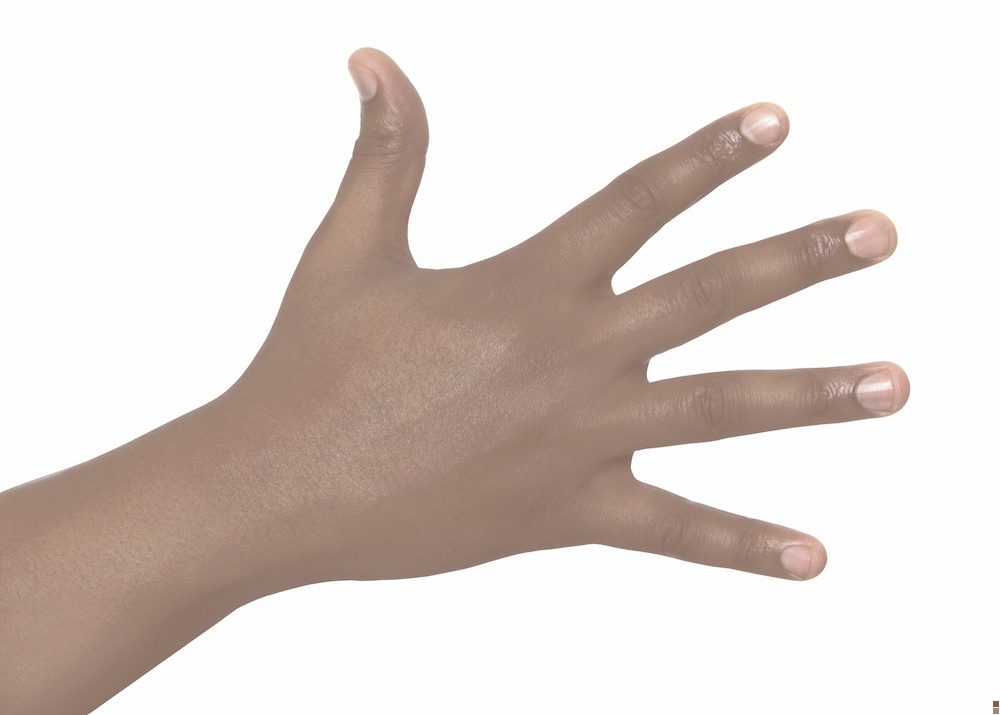
\includegraphics[width=\textwidth,height=\textheight,keepaspectratio]{../rc_test/outputs/debug/hand_dark_to_hand_pale.jpg}
  \end{minipage} \\
\hline
 \end{longtable}

\subsubsection*{Evaluation}
Images of darker skin tones and smaller changes from the original skin tone to the target colour to begin with (Row \ref{row:boost_test_hand_brown_to_hand_dark}) tend to have better results than images with large changes (Rows \ref{row:boost_test_hand_dark_to_hand_light}, \ref{row:boost_test_hand_brown_to_hand_pale}). In the case of changes towards brighter colours, this is because large changes force bright points in the original image to be truncated at white, and also causes dark regions on the image, such as shadows and grooves, to become significantly brighter and less close to true black, giving the image a ``high-key" appearance (Row \ref{row:boost_test_hand_dark_to_hand_light} and \ref{row:boost_test_hand_brown_to_hand_light}).

In addition, we noted that at this stage the transformation from a dark coloured hand to a very pale hand, or even from a mid-toned hand to a pale hand and vice versa is especially unconvincing. (Row \ref{row:boost_test_hand_brown_to_hand_pale}, also see \ref{row:boost_test_hand_dark_to_hand_pale} and \ref{row:boost_test_hand_pale_to_hand_dark})


\subsection{Proportional adjustment relative to average color}
%prop algorithm methods
To correct for the effect of the bright spots in the image being over bright and the high-key appearance resulting from all the shadows being brightened, we used an algorithm that maps the black and white points of the image to the same value, and adjusts the colours in between to match the target average colour.

\begin{algorithm}[H]
\caption{Proportional adjustment relative to average color}
\label{eq:prop_algo}
\begin{algorithmic}
\State $\mean{C_T} \gets \Call{Mean}{\vect{C_T}(U)}$
\State $\mean{C_S} \gets \Call{Mean}{\vect{C_S}(V)}$
\For{each pixel $i \in S$}
\If{$\vect{C_S}(i) \leq \mean{C_S}$}
\State $\vect{C_O}(i) \gets \displaystyle \left(\frac{\mean{C_T}}{\mean{C_S}}\right)\vect{C_S}(i)$
\Else
\State $\vect{C_O}(i) \gets \displaystyle 255 - \left(\frac{255 - \mean{C_T}}{255 - \mean{C_S}}\right)(255 - \vect{C_S}(i))$
\EndIf
\EndFor
\end{algorithmic}
\end{algorithm}

In Table \ref{tab:prop_test} we show the results for colour transfers between all possible combinations of our test images.
\begin{longtable}{|N||c|c|c|}
	\caption{Test results of brightening proportionally based on distance of color to the average.\label{tab:prop_test}}\\
	\hline
	\multicolumn{1}{|c||}{No.} & Original & Target & Results \\ 
	\hline
	    \label{row:prop_test_1} &
  \begin{minipage}{.29\textwidth}
    \includegraphics[width=\textwidth,height=\textheight,keepaspectratio]{../inputs/hand_dark.jpg}
  \end{minipage} & 
  \begin{minipage}{.29\textwidth}
    \includegraphics[width=\textwidth,height=\textheight,keepaspectratio]{../inputs/hand_brown.jpg}
  \end{minipage} & 
  \begin{minipage}{.29\textwidth}
    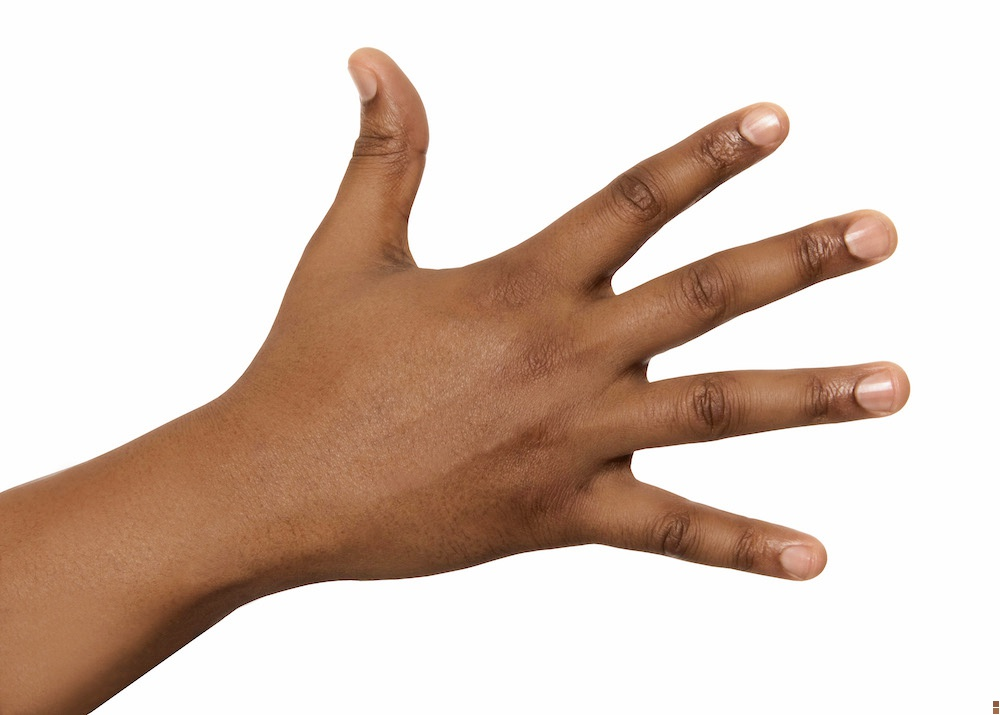
\includegraphics[width=\textwidth,height=\textheight,keepaspectratio]{../rc_test/outputs/20170516_proportional_test/hand_dark_to_hand_brown.jpg}
  \end{minipage} \\
\hline  \label{row:prop_test_1} &
  \begin{minipage}{.29\textwidth}
    \includegraphics[width=\textwidth,height=\textheight,keepaspectratio]{../inputs/hand_dark.jpg}
  \end{minipage} & 
  \begin{minipage}{.29\textwidth}
    \includegraphics[width=\textwidth,height=\textheight,keepaspectratio]{../inputs/hand_light.jpg}
  \end{minipage} & 
  \begin{minipage}{.29\textwidth}
    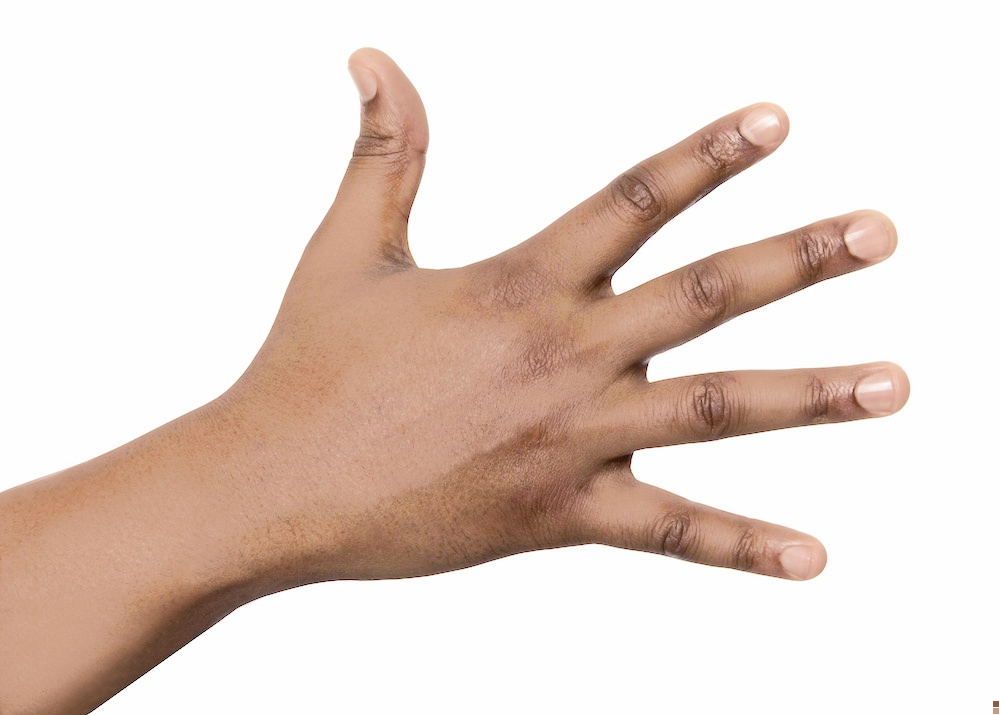
\includegraphics[width=\textwidth,height=\textheight,keepaspectratio]{../rc_test/outputs/20170516_proportional_test/hand_dark_to_hand_light.jpg}
  \end{minipage} \\
\hline  \label{row:prop_test_1} &
  \begin{minipage}{.29\textwidth}
    \includegraphics[width=\textwidth,height=\textheight,keepaspectratio]{../inputs/hand_dark.jpg}
  \end{minipage} & 
  \begin{minipage}{.29\textwidth}
    \includegraphics[width=\textwidth,height=\textheight,keepaspectratio]{../inputs/hand_pale.jpg}
  \end{minipage} & 
  \begin{minipage}{.29\textwidth}
    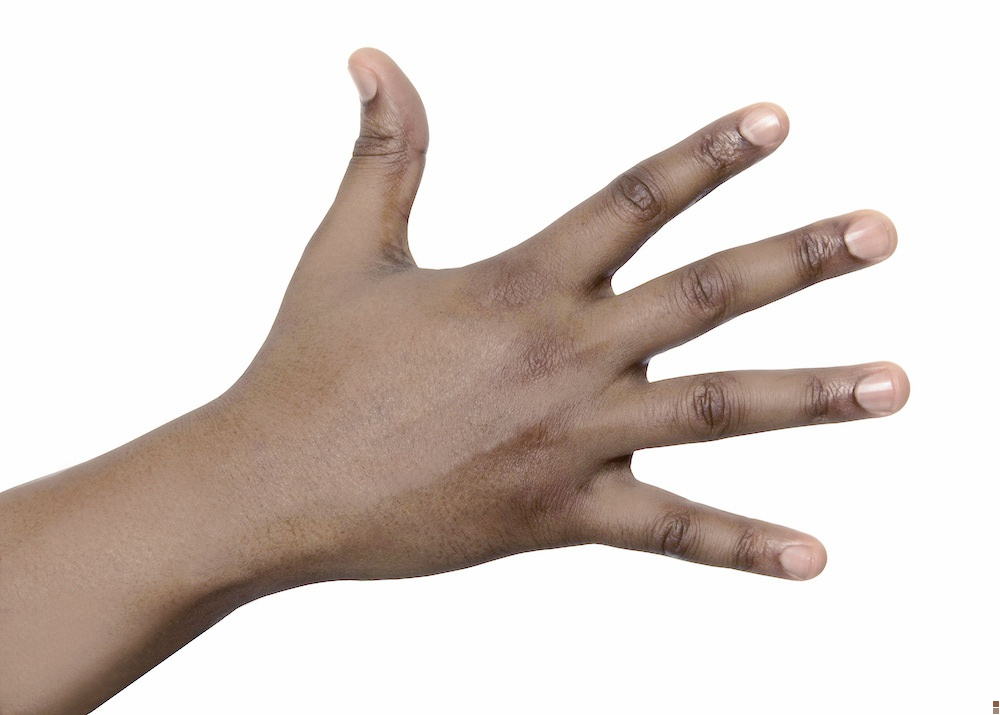
\includegraphics[width=\textwidth,height=\textheight,keepaspectratio]{../rc_test/outputs/20170516_proportional_test/hand_dark_to_hand_pale.jpg}
  \end{minipage} \\
\hline  \label{row:prop_test_1} &
  \begin{minipage}{.29\textwidth}
    \includegraphics[width=\textwidth,height=\textheight,keepaspectratio]{../inputs/hand_brown.jpg}
  \end{minipage} & 
  \begin{minipage}{.29\textwidth}
    \includegraphics[width=\textwidth,height=\textheight,keepaspectratio]{../inputs/hand_dark.jpg}
  \end{minipage} & 
  \begin{minipage}{.29\textwidth}
    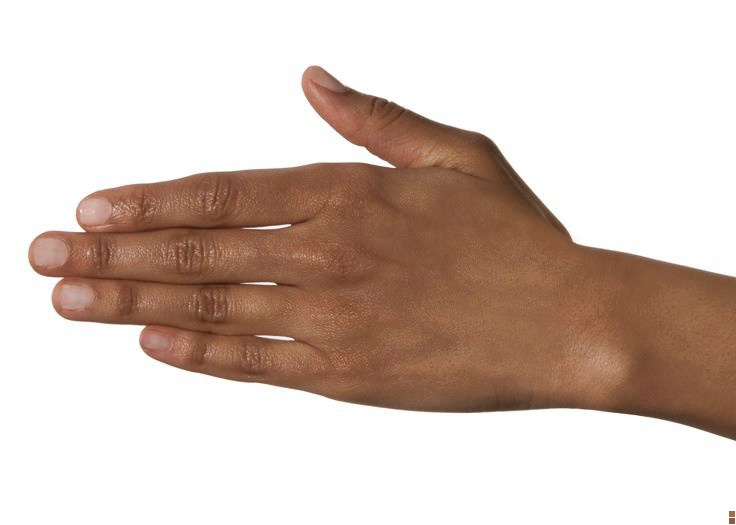
\includegraphics[width=\textwidth,height=\textheight,keepaspectratio]{../rc_test/outputs/20170516_proportional_test/hand_brown_to_hand_dark.jpg}
  \end{minipage} \\
\hline  \label{row:prop_test_1} &
  \begin{minipage}{.29\textwidth}
    \includegraphics[width=\textwidth,height=\textheight,keepaspectratio]{../inputs/hand_brown.jpg}
  \end{minipage} & 
  \begin{minipage}{.29\textwidth}
    \includegraphics[width=\textwidth,height=\textheight,keepaspectratio]{../inputs/hand_light.jpg}
  \end{minipage} & 
  \begin{minipage}{.29\textwidth}
    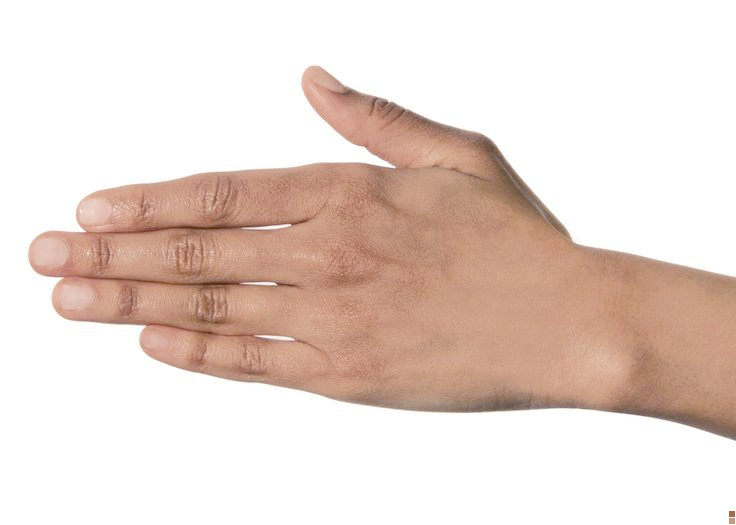
\includegraphics[width=\textwidth,height=\textheight,keepaspectratio]{../rc_test/outputs/20170516_proportional_test/hand_brown_to_hand_light.jpg}
  \end{minipage} \\
\hline  \label{row:prop_test_1} &
  \begin{minipage}{.29\textwidth}
    \includegraphics[width=\textwidth,height=\textheight,keepaspectratio]{../inputs/hand_brown.jpg}
  \end{minipage} & 
  \begin{minipage}{.29\textwidth}
    \includegraphics[width=\textwidth,height=\textheight,keepaspectratio]{../inputs/hand_pale.jpg}
  \end{minipage} & 
  \begin{minipage}{.29\textwidth}
    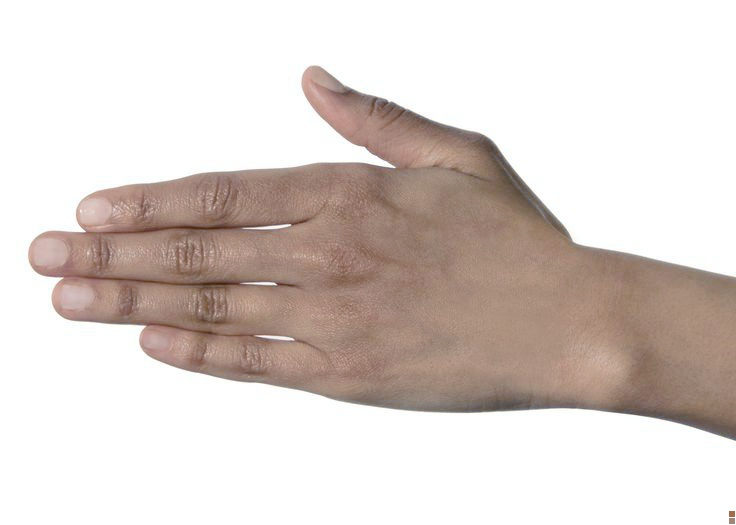
\includegraphics[width=\textwidth,height=\textheight,keepaspectratio]{../rc_test/outputs/20170516_proportional_test/hand_brown_to_hand_pale.jpg}
  \end{minipage} \\
\hline  \label{row:prop_test_1} &
  \begin{minipage}{.29\textwidth}
    \includegraphics[width=\textwidth,height=\textheight,keepaspectratio]{../inputs/hand_light.jpg}
  \end{minipage} & 
  \begin{minipage}{.29\textwidth}
    \includegraphics[width=\textwidth,height=\textheight,keepaspectratio]{../inputs/hand_dark.jpg}
  \end{minipage} & 
  \begin{minipage}{.29\textwidth}
    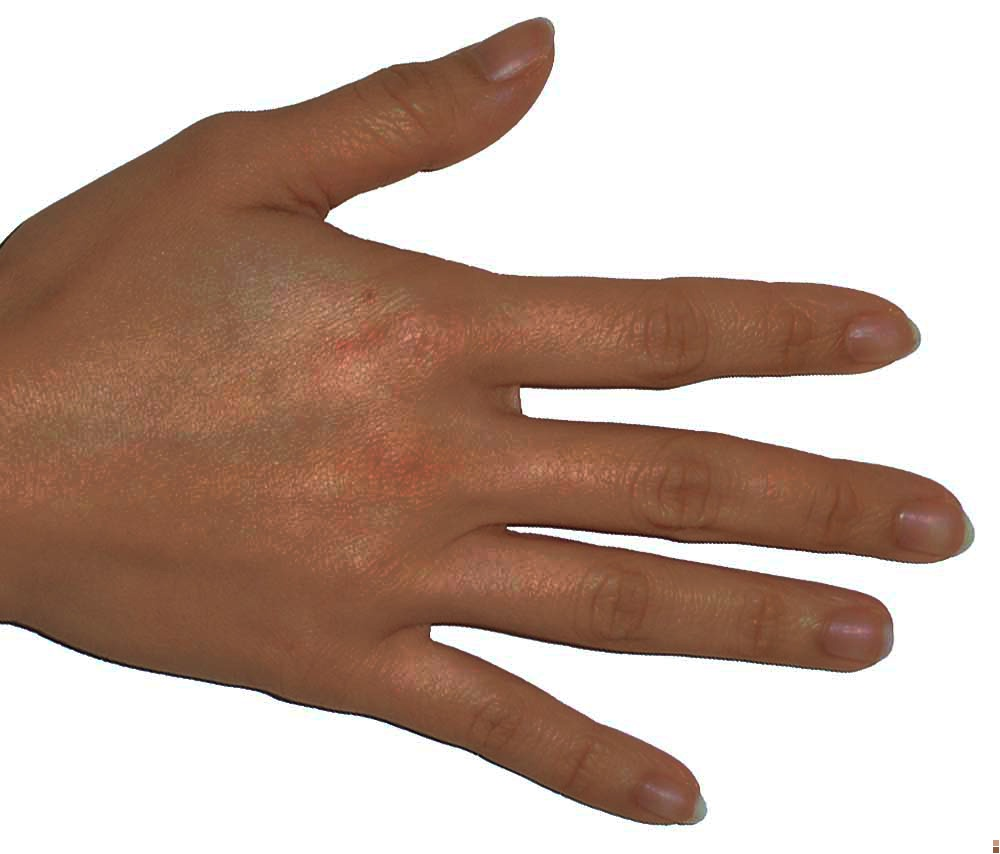
\includegraphics[width=\textwidth,height=\textheight,keepaspectratio]{../rc_test/outputs/20170516_proportional_test/hand_light_to_hand_dark.jpg}
  \end{minipage} \\
\hline  \label{row:prop_test_1} &
  \begin{minipage}{.29\textwidth}
    \includegraphics[width=\textwidth,height=\textheight,keepaspectratio]{../inputs/hand_light.jpg}
  \end{minipage} & 
  \begin{minipage}{.29\textwidth}
    \includegraphics[width=\textwidth,height=\textheight,keepaspectratio]{../inputs/hand_brown.jpg}
  \end{minipage} & 
  \begin{minipage}{.29\textwidth}
    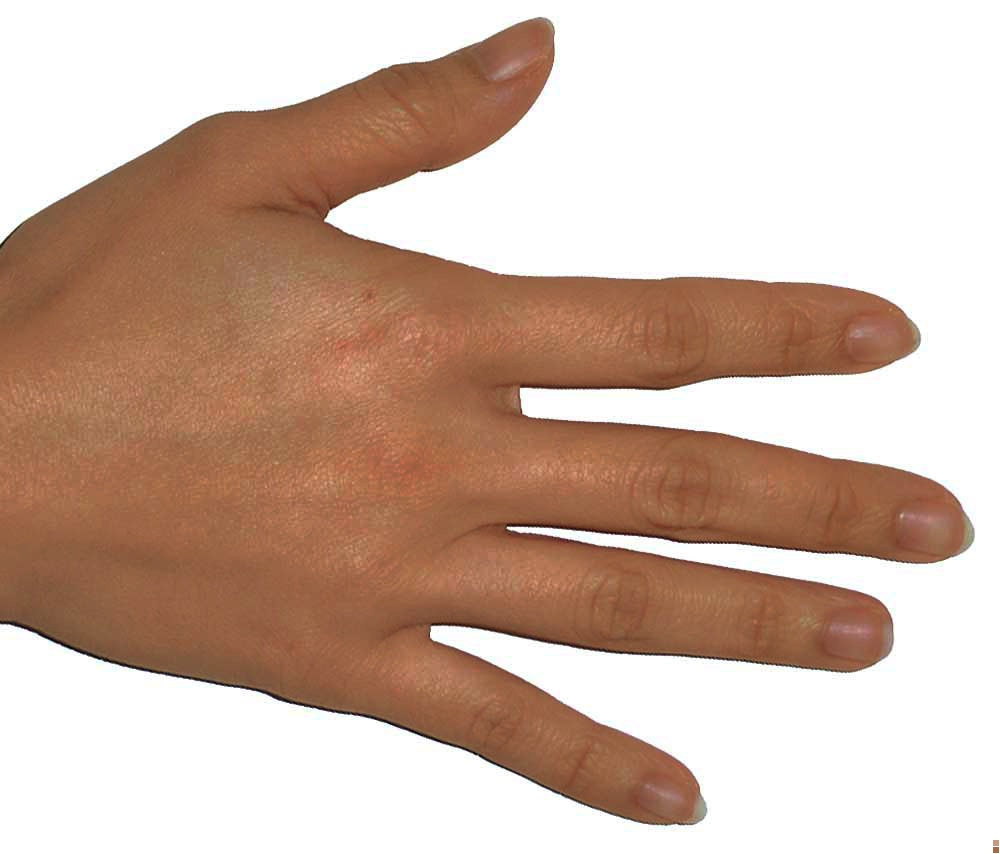
\includegraphics[width=\textwidth,height=\textheight,keepaspectratio]{../rc_test/outputs/20170516_proportional_test/hand_light_to_hand_brown.jpg}
  \end{minipage} \\
\hline  \label{row:prop_test_1} &
  \begin{minipage}{.29\textwidth}
    \includegraphics[width=\textwidth,height=\textheight,keepaspectratio]{../inputs/hand_light.jpg}
  \end{minipage} & 
  \begin{minipage}{.29\textwidth}
    \includegraphics[width=\textwidth,height=\textheight,keepaspectratio]{../inputs/hand_pale.jpg}
  \end{minipage} & 
  \begin{minipage}{.29\textwidth}
    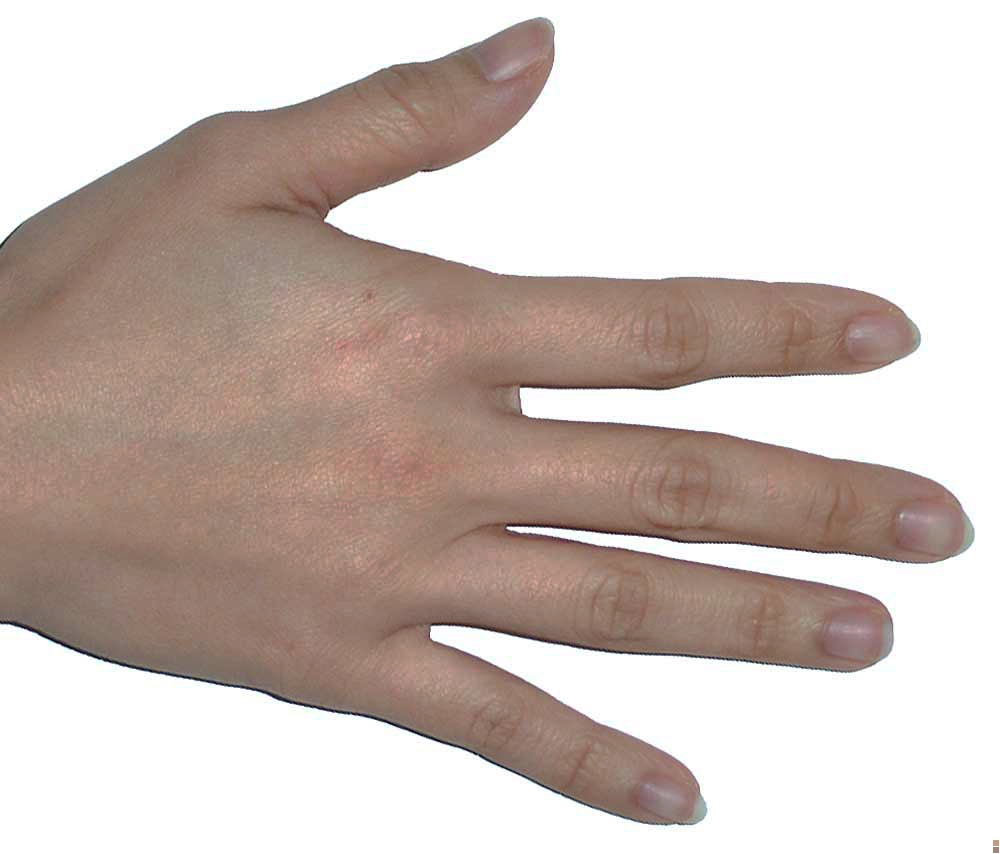
\includegraphics[width=\textwidth,height=\textheight,keepaspectratio]{../rc_test/outputs/20170516_proportional_test/hand_light_to_hand_pale.jpg}
  \end{minipage} \\
\hline  \label{row:prop_test_1} &
  \begin{minipage}{.29\textwidth}
    \includegraphics[width=\textwidth,height=\textheight,keepaspectratio]{../inputs/hand_pale.jpg}
  \end{minipage} & 
  \begin{minipage}{.29\textwidth}
    \includegraphics[width=\textwidth,height=\textheight,keepaspectratio]{../inputs/hand_dark.jpg}
  \end{minipage} & 
  \begin{minipage}{.29\textwidth}
    \includegraphics[width=\textwidth,height=\textheight,keepaspectratio]{../rc_test/outputs/20170516_proportional_test/hand_pale_to_hand_dark.jpg}
  \end{minipage} \\
\hline  \label{row:prop_test_1} &
  \begin{minipage}{.29\textwidth}
    \includegraphics[width=\textwidth,height=\textheight,keepaspectratio]{../inputs/hand_pale.jpg}
  \end{minipage} & 
  \begin{minipage}{.29\textwidth}
    \includegraphics[width=\textwidth,height=\textheight,keepaspectratio]{../inputs/hand_brown.jpg}
  \end{minipage} & 
  \begin{minipage}{.29\textwidth}
    \includegraphics[width=\textwidth,height=\textheight,keepaspectratio]{../rc_test/outputs/20170516_proportional_test/hand_pale_to_hand_brown.jpg}
  \end{minipage} \\
\hline  \label{row:prop_test_1} &
  \begin{minipage}{.29\textwidth}
    \includegraphics[width=\textwidth,height=\textheight,keepaspectratio]{../inputs/hand_pale.jpg}
  \end{minipage} & 
  \begin{minipage}{.29\textwidth}
    \includegraphics[width=\textwidth,height=\textheight,keepaspectratio]{../inputs/hand_light.jpg}
  \end{minipage} & 
  \begin{minipage}{.29\textwidth}
    \includegraphics[width=\textwidth,height=\textheight,keepaspectratio]{../rc_test/outputs/20170516_proportional_test/hand_pale_to_hand_light.jpg}
  \end{minipage} \\
\hline
 \end{longtable}

This method improved the appearance of cases with over-bright spots or ``high-key" appearance issues, as Figure \ref{img:compare_bright_spot} shows:
\begin{figure}[H]
    \centering
    \begin{subfigure}[b]{0.40\textwidth}
        \includegraphics[width=\textwidth]{../rc_test/outputs/20170516_boost_test/hand_dark_to_hand_light.jpg}
        \caption{Simple addition algorithm (Equation \ref{eq:boost_algo})result}
    \end{subfigure}
    ~
    \begin{subfigure}[b]{0.40\textwidth}
        \includegraphics[width=\textwidth]{../rc_test/outputs/20170516_proportional_test/hand_dark_to_hand_light.jpg}
        \caption{Proportional adjustment algorithm (Equation \ref{eq:prop_algo}) result}
    \end{subfigure}
    \caption{Comparison of algorithms \ref{eq:boost_algo} and \ref{eq:prop_algo} results for transforming a dark hand (Figure \ref{img:input_hands_1_dark}) to a light hand (Figure \ref{img:input_hands_1_light}).\label{img:compare_bright_spot}}
\end{figure}

We noted however, that this method noticeably does not correct for, and even exacerbates slightly relative to the simple addition algorithm the dark spots at the joints and creases of a hand of darker skin tone when it is transformed to a lighter skin tone (Row \ref{row:prop_test_hand_brown_to_hand_light}). Other results are similar to the results of the simple addition algorithm.


\subsection{Proportional adjustment with dark spot correction}
%proportional corrected algorithm methods
\subsubsection*{Algorithm}
We attempted to correct the dark spot issue by significantly reducing the absolute difference between dark pixels and the average colour, ensuring that the dark spots would instead have colours close to the average. We perform this correction on the output of the proportional adjustment algorithm.

\begin{equation} \label{eq:prop_corr_algo}
  r'' = \left.
  \begin{dcases}
    \displaystyle \mean{r'} - \frac{(\mean{r'} - r')}{\alpha}, & \text{for } r' < \mean{r'} \\
    \displaystyle r', & \text{for } r' \geq \mean{r'} \\
  \end{dcases}
  \right.\\
\end{equation}

Where $\alpha$ is a constant, $\alpha  > 1$. The same equation applies for the $g$ and $b$ channels.

\subsubsection*{Results}
See Table \ref{tab:prop_correct_test} in Appendix \ref{app:prop_corr_a10}, \ref{app:prop_corr_a5} and \ref{app:prop_corr_a3} for full results for a range of values for $\alpha$. %TODO

\subsubsection*{Evaluation}
> there are improvements for dark spots for brown to light hand as expected\\
> particularly for large alpha, there is no true black in image, so same ``high-key" effect, possibly can get rid of with another curve or peicewise func instead of straight line?
> algorithm not meant to be used on light hand to dark hand - in fact an opposite effect should be used

% \subsection{Calculation of average skin colour with brightest pixels}
% %adding correction for percentage of skin
We noticed that in the case where the target image has a pale hand and relatively dark shadows such as in Figure \ref{img:input_hands_1_light}, the average colour calculated for the target hand is too dark, causing the skin colour of the results to appear darker than the skin colour of the target. We correct this by calculating the average skin colour of the target hand with only a percentage of the brightest pixels in the original region of interest used to calculate the average. 

\begin{algorithm}[H]
\caption{Calculation of average skin colour with brightest pixels}
\label{eq:prop_corr_ave_algo}
\begin{algorithmic}
\State Let $p$ be a constant, $0 < p  < 100$
\State Let $U_p \subseteq U \subseteq T$ be the brightest $p$th percentile of pixels in $U$
\State $\mean{C_T} \gets \Call{Mean}{\vect{C_T}(U_p)}$
\end{algorithmic}
\end{algorithm}

We generated the resultant images using several different values for $p$, the percentile of brightest pixels, and determined that the $p = 10$ gave the best results, as shown in Table \ref{tab:prop_correct_test_a1p1_ave10}. In Appendices \ref{app:prop_corr_ave_a1p1_perc5} and \ref{app:prop_corr_ave_a1p1_perc25} we show the results for some other percentiles.

\begin{longtable}{|N||c|c|c|}
	\caption{Test results of proportional brightening with correction for dark spots and using brightest 10 percent of pixels to calculate average colour, $\alpha$ = 1.1\label{tab:prop_correct_test_a1p1_ave10}}\\
	\hline
	\multicolumn{1}{|c||}{No.} & Original & Target & Result \\ 
	\hline
	\input{latex_maker/prop_correct_ave_test_a1p1_perc10_label/hand_dark_to_hand_brown}
	\input{latex_maker/prop_correct_ave_test_a1p1_perc10_label/hand_dark_to_hand_light}
	\input{latex_maker/prop_correct_ave_test_a1p1_perc10_label/hand_dark_to_hand_pale}
	\input{latex_maker/prop_correct_ave_test_a1p1_perc10_label/hand_brown_to_hand_dark}
	\input{latex_maker/prop_correct_ave_test_a1p1_perc10_label/hand_brown_to_hand_light}
	\input{latex_maker/prop_correct_ave_test_a1p1_perc10_label/hand_brown_to_hand_pale}
	\input{latex_maker/prop_correct_ave_test_a1p1_perc10_label/hand_light_to_hand_dark}
	\input{latex_maker/prop_correct_ave_test_a1p1_perc10_label/hand_light_to_hand_brown}
	\input{latex_maker/prop_correct_ave_test_a1p1_perc10_label/hand_light_to_hand_pale}
	\input{latex_maker/prop_correct_ave_test_a1p1_perc10_label/hand_pale_to_hand_dark}
	\input{latex_maker/prop_correct_ave_test_a1p1_perc10_label/hand_pale_to_hand_brown}
	\input{latex_maker/prop_correct_ave_test_a1p1_perc10_label/hand_pale_to_hand_light}

 \end{longtable}

Figure \ref{img:10_perc_mask} demonstrates the new regions used to calculate the average skin colour. We can see that the areas with shadows are effectively discarded, and the average colour calculated is significantly lighter and visually more accurate to the skin colour of the target hand. 

\begin{figure}[H]
\centering
\begin{tabular}{ccc}
    \multirow{2}{*}[5em]{\begin{subfigure}[b]{0.30\textwidth}
        \includegraphics[width=\textwidth]{images/hand_pale}
        \caption{Input hand image with significant shadows}\label{img:alg_3_eval_hand_pale}
    \end{subfigure}}&
    \begin{subfigure}[b]{0.30\textwidth}
        \includegraphics[width=\textwidth]{images/pale_ave_10_original_mask}
        \caption{Mask used to calculate color in Algorithm \ref{eq:prop_corr_algo}}\label{img:original_mask}
    \end{subfigure} &
    \begin{subfigure}[b]{0.30\textwidth}
        \includegraphics[width=\textwidth]{images/ave_col_100}
        \caption{Average color calculated with Algorithm \ref{eq:prop_corr_algo}}\label{img:ave_col_100}
    \end{subfigure}\\
    &
    \begin{subfigure}[b]{0.30\textwidth}
        \includegraphics[width=\textwidth]{images/pale_ave_10_adjusted_mask}
        \caption{Mask used to calculate color in Algorithm \ref{eq:prop_corr_ave_algo}}\label{img:adjusted_mask}
    \end{subfigure} &
    \begin{subfigure}[b]{0.30\textwidth}
        \includegraphics[width=\textwidth]{images/ave_col_10}
        \caption{Average color calculated with Algorithm \ref{eq:prop_corr_ave_algo}}\label{img:ave_col_10}
    \end{subfigure}
\end{tabular}
\caption{The average color calculation process in Algorithm \ref{eq:prop_corr_ave_algo} compared to that in the previous version, Algorithm \ref{eq:prop_corr_algo}}\label{img:10_perc_mask}
\end{figure}

As a result of the more accurate target colour, the resulting output image is more accurate to the colour of the hand in the target image, as show in Figure \ref{img:compare_perc}

\begin{figure}[H]
    \centering
    \begin{subfigure}[b]{0.40\textwidth}
        \includegraphics[width=\textwidth]{../rc_test/outputs/20170522_proportional_corrected_test_alpha1p1/hand_light_to_hand_pale.jpg}
        \caption{Output obtained using all pixels for target average (Algorithm \ref{eq:prop_corr_algo})}
    \end{subfigure}
    ~
    \begin{subfigure}[b]{0.40\textwidth}
        \includegraphics[width=\textwidth]{../rc_test/outputs/20170524_prop_corr_1p1_ave_10/hand_light_to_hand_pale.jpg}
        \caption{Output obtained using brightest pixels for target average (Algorithm \ref{eq:prop_corr_ave_algo})}
    \end{subfigure}
    \caption{Comparison of Algorithms \ref{eq:prop_corr_algo} and \ref{eq:prop_corr_ave_algo} results for transforming a light hand (Figure \ref{img:input_hands_1_light}) to a pale hand (Figure \ref{img:input_hands_1_pale}).\label{img:compare_perc}}
\end{figure}

We note that, overall, the more moderate skin colour changes which use mid-toned and light hands as the source image in Rows \ref{row:prop_corr_ave_test_hand_brown_to_hand_dark} to \ref{row:prop_corr_ave_test_hand_light_to_hand_pale} now show relatively realistic and accurate results. However, for other tests with more extreme colour changes, such as in Row \ref{row:prop_corr_ave_test_hand_dark_to_hand_pale} and \ref{row:prop_corr_ave_test_hand_pale_to_hand_dark}, the colour change is still not convincing.

\pagebreak

\section{Conclusion and Future Work}
We have determined that it is feasible to produce a software that satisfies our requirements for fully automatic skin transfer for a range of skin colours starting from a hand of mid-toned skin colour. However, for a realistic appearance and for the final result to be accurate to the skin colour of the target hand, the original hand cannot have very significant skin colour differences with the target.

As a next step, we would like to improve our algorithm so that the results for transforming between large colour differences are more convincing. We would also like to optimize our results to have sufficient speed to operate on a mobile platform.
\pagebreak

\bibliographystyle{IEEEtran}
\bibliography{IEEEabrv,my_references}
\pagebreak

\appendix
\section{Results for proportional adjustment with darkspot correction, $\alpha = 1.5$}\label{app:prop_corr_ave_a1p5}
\begin{longtable}{|N||c|c|c|}
	\caption{Test results of proportional brightening with correction for dark spots, $\alpha = 1.5$\label{tab:prop_correct_test_a1p5}}\\
	\hline
	\multicolumn{1}{|c||}{No.} & Original & Target & Results \\ 
	\hline
	    \label{row:prop_correct_test_a1p5_hand_dark_to_hand_brown} &
  \begin{minipage}{.29\textwidth}
    \includegraphics[width=\textwidth,height=\textheight,keepaspectratio]{../inputs/hand_dark.jpg}
  \end{minipage} & 
  \begin{minipage}{.29\textwidth}
    \includegraphics[width=\textwidth,height=\textheight,keepaspectratio]{../inputs/hand_brown.jpg}
  \end{minipage} & 
  \begin{minipage}{.29\textwidth}
    \includegraphics[width=\textwidth,height=\textheight,keepaspectratio]{../rc_test/outputs/20170521_proportional_corrected_test_alpha1p5/hand_dark_to_hand_brown.jpg}
  \end{minipage} \\
\hline  \label{row:prop_correct_test_a1p5_hand_dark_to_hand_light} &
  \begin{minipage}{.29\textwidth}
    \includegraphics[width=\textwidth,height=\textheight,keepaspectratio]{../inputs/hand_dark.jpg}
  \end{minipage} & 
  \begin{minipage}{.29\textwidth}
    \includegraphics[width=\textwidth,height=\textheight,keepaspectratio]{../inputs/hand_light.jpg}
  \end{minipage} & 
  \begin{minipage}{.29\textwidth}
    \includegraphics[width=\textwidth,height=\textheight,keepaspectratio]{../rc_test/outputs/20170521_proportional_corrected_test_alpha1p5/hand_dark_to_hand_light.jpg}
  \end{minipage} \\
\hline  \label{row:prop_correct_test_a1p5_hand_dark_to_hand_pale} &
  \begin{minipage}{.29\textwidth}
    \includegraphics[width=\textwidth,height=\textheight,keepaspectratio]{../inputs/hand_dark.jpg}
  \end{minipage} & 
  \begin{minipage}{.29\textwidth}
    \includegraphics[width=\textwidth,height=\textheight,keepaspectratio]{../inputs/hand_pale.jpg}
  \end{minipage} & 
  \begin{minipage}{.29\textwidth}
    \includegraphics[width=\textwidth,height=\textheight,keepaspectratio]{../rc_test/outputs/20170521_proportional_corrected_test_alpha1p5/hand_dark_to_hand_pale.jpg}
  \end{minipage} \\
\hline  \label{row:prop_correct_test_a1p5_hand_brown_to_hand_dark} &
  \begin{minipage}{.29\textwidth}
    \includegraphics[width=\textwidth,height=\textheight,keepaspectratio]{../inputs/hand_brown.jpg}
  \end{minipage} & 
  \begin{minipage}{.29\textwidth}
    \includegraphics[width=\textwidth,height=\textheight,keepaspectratio]{../inputs/hand_dark.jpg}
  \end{minipage} & 
  \begin{minipage}{.29\textwidth}
    \includegraphics[width=\textwidth,height=\textheight,keepaspectratio]{../rc_test/outputs/20170521_proportional_corrected_test_alpha1p5/hand_brown_to_hand_dark.jpg}
  \end{minipage} \\
\hline  \label{row:prop_correct_test_a1p5_hand_brown_to_hand_light} &
  \begin{minipage}{.29\textwidth}
    \includegraphics[width=\textwidth,height=\textheight,keepaspectratio]{../inputs/hand_brown.jpg}
  \end{minipage} & 
  \begin{minipage}{.29\textwidth}
    \includegraphics[width=\textwidth,height=\textheight,keepaspectratio]{../inputs/hand_light.jpg}
  \end{minipage} & 
  \begin{minipage}{.29\textwidth}
    \includegraphics[width=\textwidth,height=\textheight,keepaspectratio]{../rc_test/outputs/20170521_proportional_corrected_test_alpha1p5/hand_brown_to_hand_light.jpg}
  \end{minipage} \\
\hline  \label{row:prop_correct_test_a1p5_hand_brown_to_hand_pale} &
  \begin{minipage}{.29\textwidth}
    \includegraphics[width=\textwidth,height=\textheight,keepaspectratio]{../inputs/hand_brown.jpg}
  \end{minipage} & 
  \begin{minipage}{.29\textwidth}
    \includegraphics[width=\textwidth,height=\textheight,keepaspectratio]{../inputs/hand_pale.jpg}
  \end{minipage} & 
  \begin{minipage}{.29\textwidth}
    \includegraphics[width=\textwidth,height=\textheight,keepaspectratio]{../rc_test/outputs/20170521_proportional_corrected_test_alpha1p5/hand_brown_to_hand_pale.jpg}
  \end{minipage} \\
\hline  \label{row:prop_correct_test_a1p5_hand_light_to_hand_dark} &
  \begin{minipage}{.29\textwidth}
    \includegraphics[width=\textwidth,height=\textheight,keepaspectratio]{../inputs/hand_light.jpg}
  \end{minipage} & 
  \begin{minipage}{.29\textwidth}
    \includegraphics[width=\textwidth,height=\textheight,keepaspectratio]{../inputs/hand_dark.jpg}
  \end{minipage} & 
  \begin{minipage}{.29\textwidth}
    \includegraphics[width=\textwidth,height=\textheight,keepaspectratio]{../rc_test/outputs/20170521_proportional_corrected_test_alpha1p5/hand_light_to_hand_dark.jpg}
  \end{minipage} \\
\hline  \label{row:prop_correct_test_a1p5_hand_light_to_hand_brown} &
  \begin{minipage}{.29\textwidth}
    \includegraphics[width=\textwidth,height=\textheight,keepaspectratio]{../inputs/hand_light.jpg}
  \end{minipage} & 
  \begin{minipage}{.29\textwidth}
    \includegraphics[width=\textwidth,height=\textheight,keepaspectratio]{../inputs/hand_brown.jpg}
  \end{minipage} & 
  \begin{minipage}{.29\textwidth}
    \includegraphics[width=\textwidth,height=\textheight,keepaspectratio]{../rc_test/outputs/20170521_proportional_corrected_test_alpha1p5/hand_light_to_hand_brown.jpg}
  \end{minipage} \\
\hline  \label{row:prop_correct_test_a1p5_hand_light_to_hand_pale} &
  \begin{minipage}{.29\textwidth}
    \includegraphics[width=\textwidth,height=\textheight,keepaspectratio]{../inputs/hand_light.jpg}
  \end{minipage} & 
  \begin{minipage}{.29\textwidth}
    \includegraphics[width=\textwidth,height=\textheight,keepaspectratio]{../inputs/hand_pale.jpg}
  \end{minipage} & 
  \begin{minipage}{.29\textwidth}
    \includegraphics[width=\textwidth,height=\textheight,keepaspectratio]{../rc_test/outputs/20170521_proportional_corrected_test_alpha1p5/hand_light_to_hand_pale.jpg}
  \end{minipage} \\
\hline  \label{row:prop_correct_test_a1p5_hand_pale_to_hand_dark} &
  \begin{minipage}{.29\textwidth}
    \includegraphics[width=\textwidth,height=\textheight,keepaspectratio]{../inputs/hand_pale.jpg}
  \end{minipage} & 
  \begin{minipage}{.29\textwidth}
    \includegraphics[width=\textwidth,height=\textheight,keepaspectratio]{../inputs/hand_dark.jpg}
  \end{minipage} & 
  \begin{minipage}{.29\textwidth}
    \includegraphics[width=\textwidth,height=\textheight,keepaspectratio]{../rc_test/outputs/20170521_proportional_corrected_test_alpha1p5/hand_pale_to_hand_dark.jpg}
  \end{minipage} \\
\hline  \label{row:prop_correct_test_a1p5_hand_pale_to_hand_brown} &
  \begin{minipage}{.29\textwidth}
    \includegraphics[width=\textwidth,height=\textheight,keepaspectratio]{../inputs/hand_pale.jpg}
  \end{minipage} & 
  \begin{minipage}{.29\textwidth}
    \includegraphics[width=\textwidth,height=\textheight,keepaspectratio]{../inputs/hand_brown.jpg}
  \end{minipage} & 
  \begin{minipage}{.29\textwidth}
    \includegraphics[width=\textwidth,height=\textheight,keepaspectratio]{../rc_test/outputs/20170521_proportional_corrected_test_alpha1p5/hand_pale_to_hand_brown.jpg}
  \end{minipage} \\
\hline  \label{row:prop_correct_test_a1p5_hand_pale_to_hand_light} &
  \begin{minipage}{.29\textwidth}
    \includegraphics[width=\textwidth,height=\textheight,keepaspectratio]{../inputs/hand_pale.jpg}
  \end{minipage} & 
  \begin{minipage}{.29\textwidth}
    \includegraphics[width=\textwidth,height=\textheight,keepaspectratio]{../inputs/hand_light.jpg}
  \end{minipage} & 
  \begin{minipage}{.29\textwidth}
    \includegraphics[width=\textwidth,height=\textheight,keepaspectratio]{../rc_test/outputs/20170521_proportional_corrected_test_alpha1p5/hand_pale_to_hand_light.jpg}
  \end{minipage} \\
\hline
 \end{longtable}

\section{Results for proportional adjustment with darkspot correction, $\alpha = 5$}\label{app:prop_corr_ave_a5}
\begin{longtable}{|N||c|c|c|}
	\caption{Test results of proportional brightening with correction for dark spots\label{tab:prop_correct_test_a5}}\\
	\hline
	\multicolumn{1}{|c||}{No.} & Original & Target & Results \\ 
	\hline
	    \label{row:prop_correct_test_a5_hand_dark_to_hand_brown} &
  \begin{minipage}{.29\textwidth}
    \includegraphics[width=\textwidth,height=\textheight,keepaspectratio]{../inputs/hand_dark.jpg}
  \end{minipage} & 
  \begin{minipage}{.29\textwidth}
    \includegraphics[width=\textwidth,height=\textheight,keepaspectratio]{../inputs/hand_brown.jpg}
  \end{minipage} & 
  \begin{minipage}{.29\textwidth}
    \includegraphics[width=\textwidth,height=\textheight,keepaspectratio]{../rc_test/outputs/20170517_proportional_corrected_test_alpha5/hand_dark_to_hand_brown.jpg}
  \end{minipage} \\
\hline  \label{row:prop_correct_test_a5_hand_dark_to_hand_light} &
  \begin{minipage}{.29\textwidth}
    \includegraphics[width=\textwidth,height=\textheight,keepaspectratio]{../inputs/hand_dark.jpg}
  \end{minipage} & 
  \begin{minipage}{.29\textwidth}
    \includegraphics[width=\textwidth,height=\textheight,keepaspectratio]{../inputs/hand_light.jpg}
  \end{minipage} & 
  \begin{minipage}{.29\textwidth}
    \includegraphics[width=\textwidth,height=\textheight,keepaspectratio]{../rc_test/outputs/20170517_proportional_corrected_test_alpha5/hand_dark_to_hand_light.jpg}
  \end{minipage} \\
\hline  \label{row:prop_correct_test_a5_hand_dark_to_hand_pale} &
  \begin{minipage}{.29\textwidth}
    \includegraphics[width=\textwidth,height=\textheight,keepaspectratio]{../inputs/hand_dark.jpg}
  \end{minipage} & 
  \begin{minipage}{.29\textwidth}
    \includegraphics[width=\textwidth,height=\textheight,keepaspectratio]{../inputs/hand_pale.jpg}
  \end{minipage} & 
  \begin{minipage}{.29\textwidth}
    \includegraphics[width=\textwidth,height=\textheight,keepaspectratio]{../rc_test/outputs/20170517_proportional_corrected_test_alpha5/hand_dark_to_hand_pale.jpg}
  \end{minipage} \\
\hline  \label{row:prop_correct_test_a5_hand_brown_to_hand_dark} &
  \begin{minipage}{.29\textwidth}
    \includegraphics[width=\textwidth,height=\textheight,keepaspectratio]{../inputs/hand_brown.jpg}
  \end{minipage} & 
  \begin{minipage}{.29\textwidth}
    \includegraphics[width=\textwidth,height=\textheight,keepaspectratio]{../inputs/hand_dark.jpg}
  \end{minipage} & 
  \begin{minipage}{.29\textwidth}
    \includegraphics[width=\textwidth,height=\textheight,keepaspectratio]{../rc_test/outputs/20170517_proportional_corrected_test_alpha5/hand_brown_to_hand_dark.jpg}
  \end{minipage} \\
\hline  \label{row:prop_correct_test_a5_hand_brown_to_hand_light} &
  \begin{minipage}{.29\textwidth}
    \includegraphics[width=\textwidth,height=\textheight,keepaspectratio]{../inputs/hand_brown.jpg}
  \end{minipage} & 
  \begin{minipage}{.29\textwidth}
    \includegraphics[width=\textwidth,height=\textheight,keepaspectratio]{../inputs/hand_light.jpg}
  \end{minipage} & 
  \begin{minipage}{.29\textwidth}
    \includegraphics[width=\textwidth,height=\textheight,keepaspectratio]{../rc_test/outputs/20170517_proportional_corrected_test_alpha5/hand_brown_to_hand_light.jpg}
  \end{minipage} \\
\hline  \label{row:prop_correct_test_a5_hand_brown_to_hand_pale} &
  \begin{minipage}{.29\textwidth}
    \includegraphics[width=\textwidth,height=\textheight,keepaspectratio]{../inputs/hand_brown.jpg}
  \end{minipage} & 
  \begin{minipage}{.29\textwidth}
    \includegraphics[width=\textwidth,height=\textheight,keepaspectratio]{../inputs/hand_pale.jpg}
  \end{minipage} & 
  \begin{minipage}{.29\textwidth}
    \includegraphics[width=\textwidth,height=\textheight,keepaspectratio]{../rc_test/outputs/20170517_proportional_corrected_test_alpha5/hand_brown_to_hand_pale.jpg}
  \end{minipage} \\
\hline  \label{row:prop_correct_test_a5_hand_light_to_hand_dark} &
  \begin{minipage}{.29\textwidth}
    \includegraphics[width=\textwidth,height=\textheight,keepaspectratio]{../inputs/hand_light.jpg}
  \end{minipage} & 
  \begin{minipage}{.29\textwidth}
    \includegraphics[width=\textwidth,height=\textheight,keepaspectratio]{../inputs/hand_dark.jpg}
  \end{minipage} & 
  \begin{minipage}{.29\textwidth}
    \includegraphics[width=\textwidth,height=\textheight,keepaspectratio]{../rc_test/outputs/20170517_proportional_corrected_test_alpha5/hand_light_to_hand_dark.jpg}
  \end{minipage} \\
\hline  \label{row:prop_correct_test_a5_hand_light_to_hand_brown} &
  \begin{minipage}{.29\textwidth}
    \includegraphics[width=\textwidth,height=\textheight,keepaspectratio]{../inputs/hand_light.jpg}
  \end{minipage} & 
  \begin{minipage}{.29\textwidth}
    \includegraphics[width=\textwidth,height=\textheight,keepaspectratio]{../inputs/hand_brown.jpg}
  \end{minipage} & 
  \begin{minipage}{.29\textwidth}
    \includegraphics[width=\textwidth,height=\textheight,keepaspectratio]{../rc_test/outputs/20170517_proportional_corrected_test_alpha5/hand_light_to_hand_brown.jpg}
  \end{minipage} \\
\hline  \label{row:prop_correct_test_a5_hand_light_to_hand_pale} &
  \begin{minipage}{.29\textwidth}
    \includegraphics[width=\textwidth,height=\textheight,keepaspectratio]{../inputs/hand_light.jpg}
  \end{minipage} & 
  \begin{minipage}{.29\textwidth}
    \includegraphics[width=\textwidth,height=\textheight,keepaspectratio]{../inputs/hand_pale.jpg}
  \end{minipage} & 
  \begin{minipage}{.29\textwidth}
    \includegraphics[width=\textwidth,height=\textheight,keepaspectratio]{../rc_test/outputs/20170517_proportional_corrected_test_alpha5/hand_light_to_hand_pale.jpg}
  \end{minipage} \\
\hline  \label{row:prop_correct_test_a5_hand_pale_to_hand_dark} &
  \begin{minipage}{.29\textwidth}
    \includegraphics[width=\textwidth,height=\textheight,keepaspectratio]{../inputs/hand_pale.jpg}
  \end{minipage} & 
  \begin{minipage}{.29\textwidth}
    \includegraphics[width=\textwidth,height=\textheight,keepaspectratio]{../inputs/hand_dark.jpg}
  \end{minipage} & 
  \begin{minipage}{.29\textwidth}
    \includegraphics[width=\textwidth,height=\textheight,keepaspectratio]{../rc_test/outputs/20170517_proportional_corrected_test_alpha5/hand_pale_to_hand_dark.jpg}
  \end{minipage} \\
\hline  \label{row:prop_correct_test_a5_hand_pale_to_hand_brown} &
  \begin{minipage}{.29\textwidth}
    \includegraphics[width=\textwidth,height=\textheight,keepaspectratio]{../inputs/hand_pale.jpg}
  \end{minipage} & 
  \begin{minipage}{.29\textwidth}
    \includegraphics[width=\textwidth,height=\textheight,keepaspectratio]{../inputs/hand_brown.jpg}
  \end{minipage} & 
  \begin{minipage}{.29\textwidth}
    \includegraphics[width=\textwidth,height=\textheight,keepaspectratio]{../rc_test/outputs/20170517_proportional_corrected_test_alpha5/hand_pale_to_hand_brown.jpg}
  \end{minipage} \\
\hline  \label{row:prop_correct_test_a5_hand_pale_to_hand_light} &
  \begin{minipage}{.29\textwidth}
    \includegraphics[width=\textwidth,height=\textheight,keepaspectratio]{../inputs/hand_pale.jpg}
  \end{minipage} & 
  \begin{minipage}{.29\textwidth}
    \includegraphics[width=\textwidth,height=\textheight,keepaspectratio]{../inputs/hand_light.jpg}
  \end{minipage} & 
  \begin{minipage}{.29\textwidth}
    \includegraphics[width=\textwidth,height=\textheight,keepaspectratio]{../rc_test/outputs/20170517_proportional_corrected_test_alpha5/hand_pale_to_hand_light.jpg}
  \end{minipage} \\
\hline
 \end{longtable}

\section{Complete results for proportional adjustment with darkspot correction, $\alpha = 1.1$, calculating target average color with 5th percentile bright pixels}\label{app:prop_corr_ave_a1p1_perc5}
\begin{longtable}{|N||c|c|c|}
	\caption{Test results of proportional adjusting with correction for dark spots, $\alpha = 1.1$, using brightest 5 percent of pixels for calculating target colour}\\
	\hline
	\multicolumn{1}{|c||}{No.} & Source & Target & Output \\ 
	\hline
	  \ref{row:PY_NAME_hand_dark_to_hand_brown} &
  \begin{minipage}{.29\textwidth}
    \includegraphics[width=\textwidth,height=\textheight,keepaspectratio]{../inputs/hand_dark.jpg}
  \end{minipage} & 
  \begin{minipage}{.29\textwidth}
    \includegraphics[width=\textwidth,height=\textheight,keepaspectratio]{../inputs/hand_brown.jpg}
  \end{minipage} & 
  \begin{minipage}{.29\textwidth}
    \includegraphics[width=\textwidth,height=\textheight,keepaspectratio]{../rc_test/outputs/20170524_prop_corr_1p1_ave_5/hand_dark_to_hand_brown.jpg}
  \end{minipage} \\
\hline
	  \label{row:PY_NAME_hand_dark_to_hand_light} &
  \begin{minipage}{.29\textwidth}
    \includegraphics[width=\textwidth,height=\textheight,keepaspectratio]{../inputs/hand_dark.jpg}
  \end{minipage} & 
  \begin{minipage}{.29\textwidth}
    \includegraphics[width=\textwidth,height=\textheight,keepaspectratio]{../inputs/hand_light.jpg}
  \end{minipage} & 
  \begin{minipage}{.29\textwidth}
    \includegraphics[width=\textwidth,height=\textheight,keepaspectratio]{../rc_test/outputs/20170524_prop_corr_1p1_ave_5/hand_dark_to_hand_light.jpg}
  \end{minipage} \\
\hline
	  \label{row:PY_NAME_hand_dark_to_hand_pale} &
  \begin{minipage}{.29\textwidth}
    \includegraphics[width=\textwidth,height=\textheight,keepaspectratio]{../inputs/hand_dark.jpg}
  \end{minipage} & 
  \begin{minipage}{.29\textwidth}
    \includegraphics[width=\textwidth,height=\textheight,keepaspectratio]{../inputs/hand_pale.jpg}
  \end{minipage} & 
  \begin{minipage}{.29\textwidth}
    \includegraphics[width=\textwidth,height=\textheight,keepaspectratio]{../rc_test/outputs/20170524_prop_corr_1p1_ave_5/hand_dark_to_hand_pale.jpg}
  \end{minipage} \\
\hline
	  \label{row:PY_NAME_hand_brown_to_hand_dark} &
  \begin{minipage}{.29\textwidth}
    \includegraphics[width=\textwidth,height=\textheight,keepaspectratio]{../inputs/hand_brown.jpg}
  \end{minipage} & 
  \begin{minipage}{.29\textwidth}
    \includegraphics[width=\textwidth,height=\textheight,keepaspectratio]{../inputs/hand_dark.jpg}
  \end{minipage} & 
  \begin{minipage}{.29\textwidth}
    \includegraphics[width=\textwidth,height=\textheight,keepaspectratio]{../rc_test/outputs/20170524_prop_corr_1p1_ave_10/hand_brown_to_hand_dark.jpg}
  \end{minipage} \\
\hline
	  \label{row:PY_NAME_hand_brown_to_hand_light} &
  \begin{minipage}{.29\textwidth}
    \includegraphics[width=\textwidth,height=\textheight,keepaspectratio]{../inputs/hand_brown.jpg}
  \end{minipage} & 
  \begin{minipage}{.29\textwidth}
    \includegraphics[width=\textwidth,height=\textheight,keepaspectratio]{../inputs/hand_light.jpg}
  \end{minipage} & 
  \begin{minipage}{.29\textwidth}
    \includegraphics[width=\textwidth,height=\textheight,keepaspectratio]{../rc_test/outputs/20170524_prop_corr_1p1_ave_100/hand_brown_to_hand_light.jpg}
  \end{minipage} \\
\hline
	  \ref{row:PY_NAME_hand_brown_to_hand_pale} &
  \begin{minipage}{.29\textwidth}
    \includegraphics[width=\textwidth,height=\textheight,keepaspectratio]{../inputs/hand_brown.jpg}
  \end{minipage} & 
  \begin{minipage}{.29\textwidth}
    \includegraphics[width=\textwidth,height=\textheight,keepaspectratio]{../inputs/hand_pale.jpg}
  \end{minipage} & 
  \begin{minipage}{.29\textwidth}
    \includegraphics[width=\textwidth,height=\textheight,keepaspectratio]{../rc_test/outputs/20170524_prop_corr_1p1_ave_25/hand_brown_to_hand_pale.jpg}
  \end{minipage} \\
\hline
	  \label{row:PY_NAME_hand_light_to_hand_dark} &
  \begin{minipage}{.29\textwidth}
    \includegraphics[width=\textwidth,height=\textheight,keepaspectratio]{../inputs/hand_light.jpg}
  \end{minipage} & 
  \begin{minipage}{.29\textwidth}
    \includegraphics[width=\textwidth,height=\textheight,keepaspectratio]{../inputs/hand_dark.jpg}
  \end{minipage} & 
  \begin{minipage}{.29\textwidth}
    \includegraphics[width=\textwidth,height=\textheight,keepaspectratio]{../rc_test/outputs/20170524_prop_corr_1p1_ave_5/hand_light_to_hand_dark.jpg}
  \end{minipage} \\
\hline
	  \label{row:PY_NAME_hand_light_to_hand_brown} &
  \begin{minipage}{.29\textwidth}
    \includegraphics[width=\textwidth,height=\textheight,keepaspectratio]{../inputs/hand_light.jpg}
  \end{minipage} & 
  \begin{minipage}{.29\textwidth}
    \includegraphics[width=\textwidth,height=\textheight,keepaspectratio]{../inputs/hand_brown.jpg}
  \end{minipage} & 
  \begin{minipage}{.29\textwidth}
    \includegraphics[width=\textwidth,height=\textheight,keepaspectratio]{../rc_test/outputs/20170524_prop_corr_1p1_ave_5/hand_light_to_hand_brown.jpg}
  \end{minipage} \\
\hline
	  \label{row:PY_NAME_hand_light_to_hand_pale} &
  \begin{minipage}{.29\textwidth}
    \includegraphics[width=\textwidth,height=\textheight,keepaspectratio]{../inputs/hand_light.jpg}
  \end{minipage} & 
  \begin{minipage}{.29\textwidth}
    \includegraphics[width=\textwidth,height=\textheight,keepaspectratio]{../inputs/hand_pale.jpg}
  \end{minipage} & 
  \begin{minipage}{.29\textwidth}
    \includegraphics[width=\textwidth,height=\textheight,keepaspectratio]{../rc_test/outputs/20170524_prop_corr_1p1_ave_25/hand_light_to_hand_pale.jpg}
  \end{minipage} \\
\hline
	  \ref{row:PY_NAME_hand_pale_to_hand_dark} &
  \begin{minipage}{.29\textwidth}
    \includegraphics[width=\textwidth,height=\textheight,keepaspectratio]{../inputs/hand_pale.jpg}
  \end{minipage} & 
  \begin{minipage}{.29\textwidth}
    \includegraphics[width=\textwidth,height=\textheight,keepaspectratio]{../inputs/hand_dark.jpg}
  \end{minipage} & 
  \begin{minipage}{.29\textwidth}
    \includegraphics[width=\textwidth,height=\textheight,keepaspectratio]{../rc_test/outputs/20170524_prop_corr_1p1_ave_5/hand_pale_to_hand_dark.jpg}
  \end{minipage} \\
\hline
	  \ref{row:PY_NAME_hand_pale_to_hand_brown} &
  \begin{minipage}{.29\textwidth}
    \includegraphics[width=\textwidth,height=\textheight,keepaspectratio]{../inputs/hand_pale.jpg}
  \end{minipage} & 
  \begin{minipage}{.29\textwidth}
    \includegraphics[width=\textwidth,height=\textheight,keepaspectratio]{../inputs/hand_brown.jpg}
  \end{minipage} & 
  \begin{minipage}{.29\textwidth}
    \includegraphics[width=\textwidth,height=\textheight,keepaspectratio]{../rc_test/outputs/20170524_prop_corr_1p1_ave_100/hand_pale_to_hand_brown.jpg}
  \end{minipage} \\
\hline
	  \ref{row:PY_NAME_hand_pale_to_hand_light} &
  \begin{minipage}{.29\textwidth}
    \includegraphics[width=\textwidth,height=\textheight,keepaspectratio]{../inputs/hand_pale.jpg}
  \end{minipage} & 
  \begin{minipage}{.29\textwidth}
    \includegraphics[width=\textwidth,height=\textheight,keepaspectratio]{../inputs/hand_light.jpg}
  \end{minipage} & 
  \begin{minipage}{.29\textwidth}
    \includegraphics[width=\textwidth,height=\textheight,keepaspectratio]{../rc_test/outputs/20170524_prop_corr_1p1_ave_100/hand_pale_to_hand_light.jpg}
  \end{minipage} \\
\hline

 \end{longtable}

\section{Complete results for proportional adjustment with darkspot correction, $\alpha = 1.1$, calculating target average color with 25th percentile bright pixels}\label{app:prop_corr_ave_a1p1_perc25}
\begin{longtable}{|N||c|c|c|}
	\caption{Test results of proportional adjusting with correction for dark spots, $\alpha = 1.1$, using brightest 25 percent of pixels for calculating target colour}\\
	\hline
	\multicolumn{1}{|c||}{No.} & Source & Target & Output \\ 
	\hline
	  \ref{row:PY_NAME_hand_dark_to_hand_brown} &
  \begin{minipage}{.29\textwidth}
    \includegraphics[width=\textwidth,height=\textheight,keepaspectratio]{../inputs/hand_dark.jpg}
  \end{minipage} & 
  \begin{minipage}{.29\textwidth}
    \includegraphics[width=\textwidth,height=\textheight,keepaspectratio]{../inputs/hand_brown.jpg}
  \end{minipage} & 
  \begin{minipage}{.29\textwidth}
    \includegraphics[width=\textwidth,height=\textheight,keepaspectratio]{../rc_test/outputs/20170524_prop_corr_1p1_ave_5/hand_dark_to_hand_brown.jpg}
  \end{minipage} \\
\hline
	  \label{row:PY_NAME_hand_dark_to_hand_light} &
  \begin{minipage}{.29\textwidth}
    \includegraphics[width=\textwidth,height=\textheight,keepaspectratio]{../inputs/hand_dark.jpg}
  \end{minipage} & 
  \begin{minipage}{.29\textwidth}
    \includegraphics[width=\textwidth,height=\textheight,keepaspectratio]{../inputs/hand_light.jpg}
  \end{minipage} & 
  \begin{minipage}{.29\textwidth}
    \includegraphics[width=\textwidth,height=\textheight,keepaspectratio]{../rc_test/outputs/20170524_prop_corr_1p1_ave_5/hand_dark_to_hand_light.jpg}
  \end{minipage} \\
\hline
	  \label{row:PY_NAME_hand_dark_to_hand_pale} &
  \begin{minipage}{.29\textwidth}
    \includegraphics[width=\textwidth,height=\textheight,keepaspectratio]{../inputs/hand_dark.jpg}
  \end{minipage} & 
  \begin{minipage}{.29\textwidth}
    \includegraphics[width=\textwidth,height=\textheight,keepaspectratio]{../inputs/hand_pale.jpg}
  \end{minipage} & 
  \begin{minipage}{.29\textwidth}
    \includegraphics[width=\textwidth,height=\textheight,keepaspectratio]{../rc_test/outputs/20170524_prop_corr_1p1_ave_5/hand_dark_to_hand_pale.jpg}
  \end{minipage} \\
\hline
	  \label{row:PY_NAME_hand_brown_to_hand_dark} &
  \begin{minipage}{.29\textwidth}
    \includegraphics[width=\textwidth,height=\textheight,keepaspectratio]{../inputs/hand_brown.jpg}
  \end{minipage} & 
  \begin{minipage}{.29\textwidth}
    \includegraphics[width=\textwidth,height=\textheight,keepaspectratio]{../inputs/hand_dark.jpg}
  \end{minipage} & 
  \begin{minipage}{.29\textwidth}
    \includegraphics[width=\textwidth,height=\textheight,keepaspectratio]{../rc_test/outputs/20170524_prop_corr_1p1_ave_10/hand_brown_to_hand_dark.jpg}
  \end{minipage} \\
\hline
	  \label{row:PY_NAME_hand_brown_to_hand_light} &
  \begin{minipage}{.29\textwidth}
    \includegraphics[width=\textwidth,height=\textheight,keepaspectratio]{../inputs/hand_brown.jpg}
  \end{minipage} & 
  \begin{minipage}{.29\textwidth}
    \includegraphics[width=\textwidth,height=\textheight,keepaspectratio]{../inputs/hand_light.jpg}
  \end{minipage} & 
  \begin{minipage}{.29\textwidth}
    \includegraphics[width=\textwidth,height=\textheight,keepaspectratio]{../rc_test/outputs/20170524_prop_corr_1p1_ave_100/hand_brown_to_hand_light.jpg}
  \end{minipage} \\
\hline
	  \ref{row:PY_NAME_hand_brown_to_hand_pale} &
  \begin{minipage}{.29\textwidth}
    \includegraphics[width=\textwidth,height=\textheight,keepaspectratio]{../inputs/hand_brown.jpg}
  \end{minipage} & 
  \begin{minipage}{.29\textwidth}
    \includegraphics[width=\textwidth,height=\textheight,keepaspectratio]{../inputs/hand_pale.jpg}
  \end{minipage} & 
  \begin{minipage}{.29\textwidth}
    \includegraphics[width=\textwidth,height=\textheight,keepaspectratio]{../rc_test/outputs/20170524_prop_corr_1p1_ave_25/hand_brown_to_hand_pale.jpg}
  \end{minipage} \\
\hline
	  \label{row:PY_NAME_hand_light_to_hand_dark} &
  \begin{minipage}{.29\textwidth}
    \includegraphics[width=\textwidth,height=\textheight,keepaspectratio]{../inputs/hand_light.jpg}
  \end{minipage} & 
  \begin{minipage}{.29\textwidth}
    \includegraphics[width=\textwidth,height=\textheight,keepaspectratio]{../inputs/hand_dark.jpg}
  \end{minipage} & 
  \begin{minipage}{.29\textwidth}
    \includegraphics[width=\textwidth,height=\textheight,keepaspectratio]{../rc_test/outputs/20170524_prop_corr_1p1_ave_5/hand_light_to_hand_dark.jpg}
  \end{minipage} \\
\hline
	  \label{row:PY_NAME_hand_light_to_hand_brown} &
  \begin{minipage}{.29\textwidth}
    \includegraphics[width=\textwidth,height=\textheight,keepaspectratio]{../inputs/hand_light.jpg}
  \end{minipage} & 
  \begin{minipage}{.29\textwidth}
    \includegraphics[width=\textwidth,height=\textheight,keepaspectratio]{../inputs/hand_brown.jpg}
  \end{minipage} & 
  \begin{minipage}{.29\textwidth}
    \includegraphics[width=\textwidth,height=\textheight,keepaspectratio]{../rc_test/outputs/20170524_prop_corr_1p1_ave_5/hand_light_to_hand_brown.jpg}
  \end{minipage} \\
\hline
	  \label{row:PY_NAME_hand_light_to_hand_pale} &
  \begin{minipage}{.29\textwidth}
    \includegraphics[width=\textwidth,height=\textheight,keepaspectratio]{../inputs/hand_light.jpg}
  \end{minipage} & 
  \begin{minipage}{.29\textwidth}
    \includegraphics[width=\textwidth,height=\textheight,keepaspectratio]{../inputs/hand_pale.jpg}
  \end{minipage} & 
  \begin{minipage}{.29\textwidth}
    \includegraphics[width=\textwidth,height=\textheight,keepaspectratio]{../rc_test/outputs/20170524_prop_corr_1p1_ave_25/hand_light_to_hand_pale.jpg}
  \end{minipage} \\
\hline
	  \ref{row:PY_NAME_hand_pale_to_hand_dark} &
  \begin{minipage}{.29\textwidth}
    \includegraphics[width=\textwidth,height=\textheight,keepaspectratio]{../inputs/hand_pale.jpg}
  \end{minipage} & 
  \begin{minipage}{.29\textwidth}
    \includegraphics[width=\textwidth,height=\textheight,keepaspectratio]{../inputs/hand_dark.jpg}
  \end{minipage} & 
  \begin{minipage}{.29\textwidth}
    \includegraphics[width=\textwidth,height=\textheight,keepaspectratio]{../rc_test/outputs/20170524_prop_corr_1p1_ave_5/hand_pale_to_hand_dark.jpg}
  \end{minipage} \\
\hline
	  \ref{row:PY_NAME_hand_pale_to_hand_brown} &
  \begin{minipage}{.29\textwidth}
    \includegraphics[width=\textwidth,height=\textheight,keepaspectratio]{../inputs/hand_pale.jpg}
  \end{minipage} & 
  \begin{minipage}{.29\textwidth}
    \includegraphics[width=\textwidth,height=\textheight,keepaspectratio]{../inputs/hand_brown.jpg}
  \end{minipage} & 
  \begin{minipage}{.29\textwidth}
    \includegraphics[width=\textwidth,height=\textheight,keepaspectratio]{../rc_test/outputs/20170524_prop_corr_1p1_ave_100/hand_pale_to_hand_brown.jpg}
  \end{minipage} \\
\hline
	  \ref{row:PY_NAME_hand_pale_to_hand_light} &
  \begin{minipage}{.29\textwidth}
    \includegraphics[width=\textwidth,height=\textheight,keepaspectratio]{../inputs/hand_pale.jpg}
  \end{minipage} & 
  \begin{minipage}{.29\textwidth}
    \includegraphics[width=\textwidth,height=\textheight,keepaspectratio]{../inputs/hand_light.jpg}
  \end{minipage} & 
  \begin{minipage}{.29\textwidth}
    \includegraphics[width=\textwidth,height=\textheight,keepaspectratio]{../rc_test/outputs/20170524_prop_corr_1p1_ave_100/hand_pale_to_hand_light.jpg}
  \end{minipage} \\
\hline

 \end{longtable}

\end{document}